%%%%%%%%%%%%%%%%%%%%%%%%%%%%%%%%%%%%%%%%%%%%%%%%%%%%%%%%%%%
% Dokumentinformationen                                   %
%%%%%%%%%%%%%%%%%%%%%%%%%%%%%%%%%%%%%%%%%%%%%%%%%%%%%%%%%%%
\title{Mobkom AP Zusammenfassung}
\author{D. Bargen, G. Dengler}

\documentclass[10pt,twoside,a4paper,fleqn]{article}
\include{header/zusammenfassung}
% Header

% \input macht keine neue Seiteß% \include macht eine neue Seite

\usepackage{tikz}
\usetikzlibrary{fit}
\usepackage{circuitikz}
\usepackage{enumitem}
\usepackage{booktabs}
\setlist{noitemsep,topsep=0pt,parsep=0pt,partopsep=0pt}
\usepackage{textcomp} % Für Grad zeichen

\setlength{\mathindent}{0pt}
\raggedbottom
\begin{document}

\begin{titlepage}
	\maketitle

	\vspace{100mm}

	%\includegraphics{hsr_logo.png}
	\thispagestyle{empty} % Don't start page numbers on this page
\end{titlepage}
\setcounter{tocdepth}{2}
\tableofcontents 

\newpage

\section{Einführung in die Mobilkommunikation}
\subsection{Mobkom The Player}

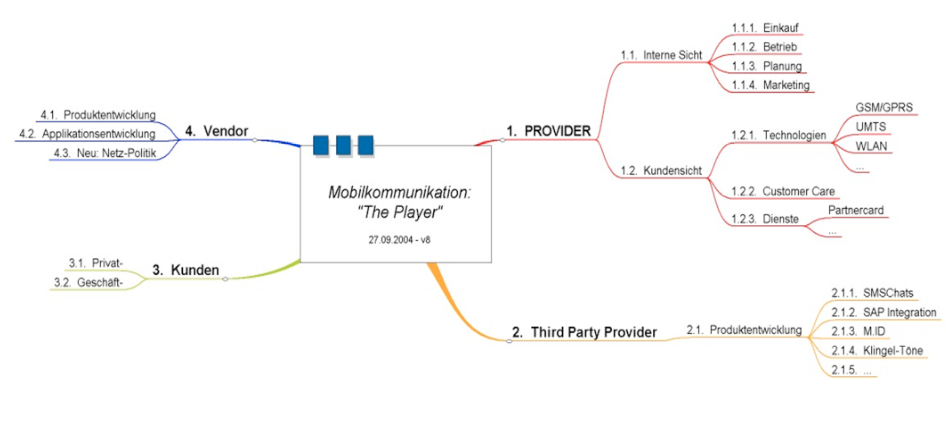
\includegraphics[height = 5 cm]{./Pics/MobKomThePlayer}

\subsection{Mobkom Generell}
\begin{minipage}{0.5 \linewidth}
\begin{itemize}
\item sicherheitskritisches 
\item simultan laufendes
\item Echtzeit
\item Zeit abweichendes
\item non-stop
\item Fehlertolerantes
\item  uneinheitliches
\item dezentrales System
\end{itemize}
\end{minipage}
\begin{minipage}{0.5 \linewidth}
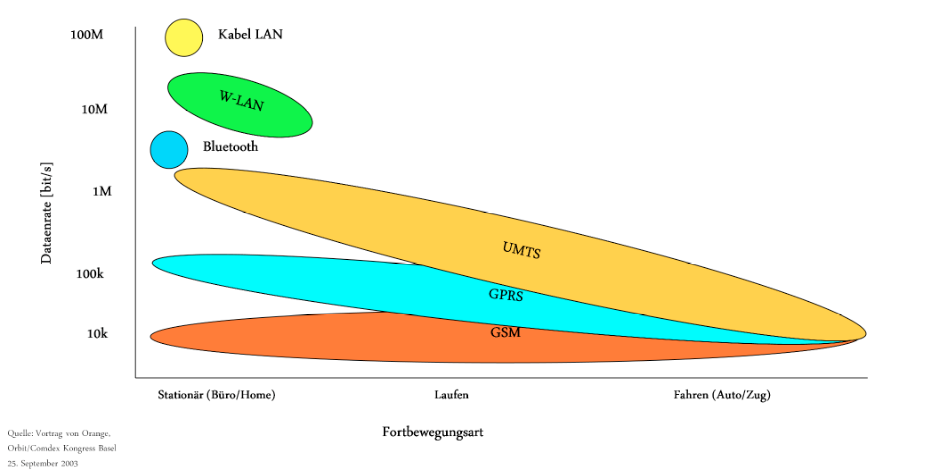
\includegraphics[width = \linewidth]{./Pics/Technologien}
\end{minipage}

\subsection{Multiplexing}
\subsubsection{Raum-Multiplex}
Raum wird in verschiedene Bereiche aufgeteilt und jedem Konkurrenten/Teilnehmer ein Bereich zugewisen, so dsas diese sich bei zeitgleicher Nutzung nicht gegenseiteig beeinflussen können. \\
\textbf{Beispiel :} Mobilfunk-Zellenaufteilung, Kabelbündel

\subsubsection{Zeit-Multiplex TDMA}
Das Medium der Kommunikation darf von jedem Konkurrenten exklusiv für eine bestimmte Periode genutzt werden (Zeitabschnitt wird zugewiesen, fest oder zufällig je nach Bedarf) \\
\textbf{Beispiel :} Festnetzte,GSM,IEEE 802,3 (CSMA/CD)

\subsubsection{Frequenz-Muliplex FDMA}
Jedem Konkurrenten um das MEdium wird eine exklusive Frequenz zugewiesen, auf der er dann zeitgleich mit den anderen senden kann.
\textbf{Beispiel :} Radio-/TV-Frequenz, GSM-Netz, Betriebsfunknetze,Glasfasernetze

\subsubsection{Code-Multiplex CDMA}
Zuordnung exklusiver Codes zu einzelnen Sendern, so dass alle gleichzeitig auf einer identischen Frequenz senden können, aber anhand des Codes eindeutig identifiziert werden können.
\textbf{Beispiel :} UMTS

\subsection{Störung}
\subsubsection{Abschattung}
Durch Hindernisse kann ein Signal abgeschattet (shadowing) werden. Der Empfang wird dadurch erschwert oder verhindert
\textbf{Beispiel :} Hochhäuser, Tunnel

\subsubsection{Reflexion}
Wellenförmiges Signal wird an grosser Fläche (spiegelartig) reflektiert. Reflektierte Signale sind schwächer als direkt empfangene (wenn sie denn überhaupt empfangen werden)

\subsubsection{Streuung}
Relativ kleine Hindernisse können das Signal streuen (scattering), das sich dann in verschiedene Richtungen weiterbewegt.

\subsubsection{Beugung}
Kanten können eine Beugung (diffraction)/Ablenkung des Signals verursachen.

\subsubsection{Dämpfung \& Verzögerung}
Empfangsleistung nimmt proportional zum Quadrat der Entfernung zwischen Sender und Empfänger ab(path loss). Zeitrahmensynchronisation ist ortsabhängig (time alginment)

\subsubsection{Interferenzen}
Konkurrieren mehrer Mobilstationen um das Übertragungsmedium können Interferenzen (Überlagerung zwischen getrennten Kanälen) auftreten.

\subsubsection{Mehrwegausbreitung-Multipath Fading}
\begin{itemize}
\item Aufgrund von Streuung, Beugung und REflexion kann das Signal das Ziel auf unterschiedlichen Wegen erreichen.
\item Der Impuls des Senders kann beim Empfänger mehrfach und zeitlich versetzt auftreten.
\item Die Stärke der eingehenden Signale schwankt, da die Ausbreitungswege unterschiedliche Dämpfung aufweisen können.
\item Unterschieden wird zwischen 
\begin{itemize}
\item Rayleigh Fading 
\item Time Dispersion
\end{itemize}
\end{itemize}

\subsection{Zellplanung}
Die Zentrale frage ist, wie viele Zellen werden für die Netzabdeckung der Region benötigt. Die Zellplanung ist abhängig von:
\begin{itemize}
\item Anzahl Kanäle pro Zelle
\item die mittlere Anzahl der Teilnehmer pro Zelle (steuerbar über die grösse der Zelle)
\item Qualität des angebotenen Dienstes (Grade Of Service GOS)
\item der mittlere Verkehr, den die Teilnehmer pro Zelle produzieren, ist abhängig von der
\begin{itemize}
\item Populationsverteilung
\item Verteilung Autobenutzung
\item Verteilung des Einkommens in der Region
\item Charakteristik der landestypischen Telefonierverhaltens 
\item Telefonstatistik
\item Anzahl der Kunden (subscriber) des Mobilfunkanbieters
\end{itemize}
\end{itemize}
\begin{multicols}{2}
\begin{eqnarray}
A = \frac{n \cdot T}{3600 s} \\
\left[ A \right] = \frac{\left[ s \right] }{\left[ s \right] } = \text{Pseudoeinheit Erlang} \\
B = \frac{\frac{A^n}{n!}}{\sum_{i = 0}^{n} \frac{A^i}{i!}}
\end{eqnarray}
\columnbreak

In 1 und 2:
\begin{itemize}
\item A = Angebotener Verkehr
\item n = mittlere Anzahl der Anrufe pro Zelle
\item T = mittlere Dauer eines Gespräches
\end{itemize}
In 3:
\begin{itemize}
\item A = Angebotener Verkehr zur Hauptverkehrsstunde
\item n  = Anzahl Kanäle
\item B = Blockierwahrscheinlichkeit
\end{itemize}
\end{multicols}
\subsubsection{Verlustsysteme}

Reine Wartesysteme existieren in der Praxis nicht. Jedoch kann mit Annäherungen gearbeitet werden, wenn die Anzahl zur Verfügung stehenden Warteplätze gegenüber der mittleren Warteschlangenlänge ausreichend gross ist. \\

Die Verlustwahrscheinlichkeit lässt sich mit der Erlang B Funktion berechnen. Die Formel ist oben und die Verlustwahrscheinlichkeit ist gleich der Blockierwahrscheinlichkeit.


\newpage
\section{GSM - Global System for Mobile Communications}
\subsection{Einführung}
\subsubsection{Netze}
\begin{itemize}
\item A-Netz (1958 - 1976)
\begin{itemize}
\item Handvermittlung
\item sehr teure Endgeräte
\item Kapazitätsgrenzen (Rufnummerngrenzen)
\item Höchstteilnehmerzahl 11000(1971)
\end{itemize}
\item B/B2-Netz(1972-1994)
\begin{itemize}
\item Selbstwahl ab 1977 Übernahme von A-Frequenzen durch
\item B2-Netz
\item keine einheitliche Vorwahl(genauer Standort musst bekannt sein)
\item Höchstteilnehmerzahl 27000 (1986)
\end{itemize}
\item C-Netz (1985-)
\begin{itemize}
\item Analoges Mobilfunknetz
\item Selbstwahl mit Handover
\item Einheitliche Vorwahl 0161
\item Dienste
\end{itemize}
\item D-Netz
\begin{itemize}
\item Ziel war neues Netz
\begin{itemize}
\item Subjektiv gute Sprachqualität
\item Hohe Sicherheit
\item Preisgünstige Endgeräte, niedrige Betriebskosten
\item Internationales Roaming
\item Unterstütung von Handgeräten
\item Unterstützung neuartiger Dienste
\item ISDN Kompabilität
\item 1989 wurd die Verantwortung für GSM an das ETSI übertragen, 1990 wurden Spezifikationen publiziert
\end{itemize}
\item 1990 Abschluss der Standardisierung 
\item 1992 Kommerzieller Start des ersten GSM Netztes (T-D1)
\item 1993 Neudefinition für GSM (SAM 900,1800 und 1900(USA))
\item 1995 Weltweit 120 GSM-Netze 
\item 1998 Über 200 GSM-Netzbetreiber in über 110 Ländern
\end{itemize}
\end{itemize}

\subsection{Netzstruktur und Aufbau}
\begin{itemize}
\item Multiplexing
\begin{itemize}
\item Raummultiplex - Netzstruktur und Aufbau
\item Frequenzmultiplex - Frequenzplan
\item Zeitmultiplex - Rahmenstruktur und Kanalplanung
\end{itemize}
\item Übertragungsprobleme
\begin{itemize}
\item Bitfehlerrate - Kanalcodierung
\item Rayliegh Fading - Frequenzy Hopping
\item Time Dispersion - Adaptive Equalization
\item Rahmensynchronisation - Timing Advance
\end{itemize}
\item Architektur
\begin{itemize}
\item Kanalstruktur
\item Protokollstack
\end{itemize}
\item Verhalten
\begin{itemize}
\item Anmelden, Abmelden
\item Sicherheitsprotokoll
\item Verbindungsauf- und abbbau
\item Verbindungssteuerung
\end{itemize}
\end{itemize}

\subsection{Multiplextechnik}
\subsubsection{Raummultiplex durch Zellen}
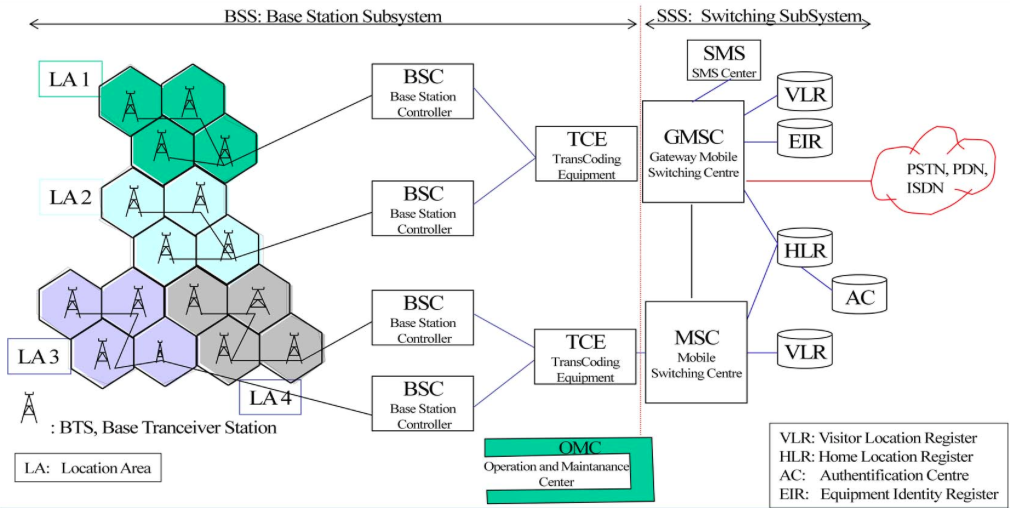
\includegraphics[width = \linewidth]{./Pics/GSMZellen}

\begin{itemize}
\item Wiederverwendung der Frequenz
\item Unterschiedliche Zelltypen
\begin{itemize}
\item Macro Cell
\item Micro Cell
\item Pico Cell
\item Femto Cell
\item Sectorized Cell
\item Umbrella Cell
\item Extended Cell
\end{itemize}
\item Einsatz der Zelltypen verkehrsabhängig, siehe auch Verlustsysteme und Grade of Service (GOS)
\item für die Planung wird pro Zelle ein Verkehr von 25 - 35 mErlang und ein GOS von 2\% veranschlagt
\end{itemize}
\vspace{0.5 cm}
\begin{minipage}{0.7 \linewidth}
\begin{itemize}
\item Pico-Zelle
\begin{itemize}
\item Maximale Reichweite 100m
\item Inhouse sowie Gebäude- und Grundstückversorgung
\end{itemize}
\item Micro-Zelle
\begin{itemize}
\item Reichweite 100m bis 2 km
\item Hohes Verkehrsaufkommen
\end{itemize}
\item Macro-Zelle
\begin{itemize}
\item Reichweite 2 km bis 35 km
\item Schnelle Abdeckung grosser Gebiete 
\item Gernges Verkehrsaufkommen
\item Verwendung als Schirm über Micro-Zellen
\end{itemize}
\item Sektorisierte Zelle
\begin{itemize}
\item Ein Aufbauort (site) zur Realisierung der Sektorzellen
\item Hier werden mehrere BTS zusammengestellt
\item Dienen zur Abdeckung von Gebieten mit hohem erwartetem Verkehrsaufkommen
\end{itemize}
\end{itemize}
\end{minipage}
\begin{minipage}{0.3 \linewidth}
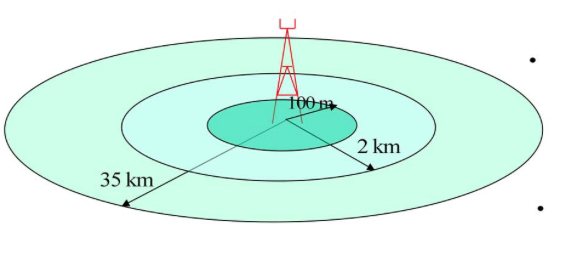
\includegraphics[width = \linewidth]{./Pics/GSMZellen2}
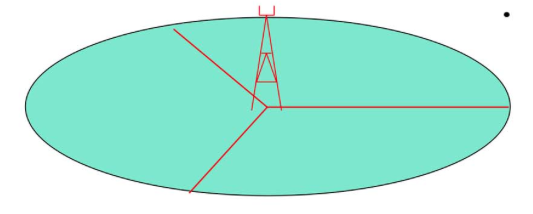
\includegraphics[width = \linewidth]{./Pics/GSMZellen3}
\end{minipage}
\begin{minipage}{0.5 \linewidth}
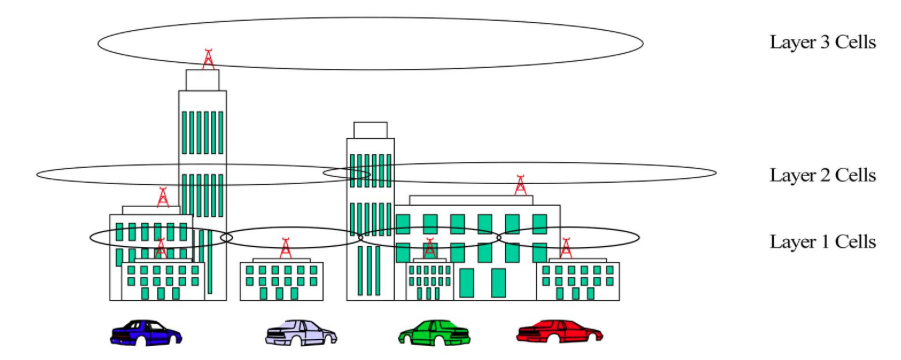
\includegraphics[width = \linewidth]{./Pics/GSMZellenPrinzip}
\end{minipage}
\begin{minipage}{0.5 \linewidth}
\begin{itemize}
\item Die Zellen werden nach Bewegungsgeschwindigkeit des User gewählt
\item So können unnötig viele Zellenwechsel verhindert werden
\item In Ballungsgebieten, in denen sich viele User auf kleinem Raum befinden und nicht grossartig Bewegen, kann man Layer 1 Zellen mehr Bandbreite zu Verfügung stellen
\end{itemize}
\end{minipage}

\subsubsection{Frequenzmultiplex}
\begin{minipage}{0.5 \linewidth}
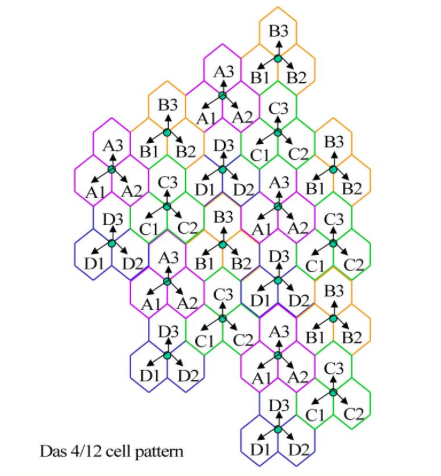
\includegraphics[width = \linewidth]{./Pics/GSMFrequenzplan}
\end{minipage}
\begin{minipage}{0.5 \linewidth}
\begin{itemize}
\item Gruppen von Frequenzen werden zu so genannten Clustern zusammengefasst
\item Aus Interferenz-gründen ist der Abstand zwischen wieder benutzten Frequenzen so gross wie möglich zu halten. Durch Clustering wird dies einfach realisiert
\item Für GSM werden die 3/9 oder 4/12 Re-Use-Pattern empfohlen
\end{itemize}
\end{minipage}
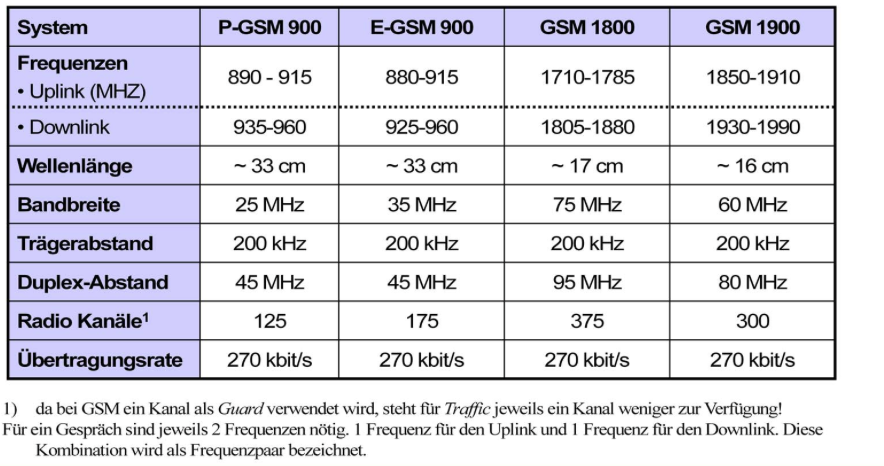
\includegraphics[width = 0.5 \linewidth]{./Pics/GSMFrequenzkonzept}

\subsubsection{Zeitmultiplex}

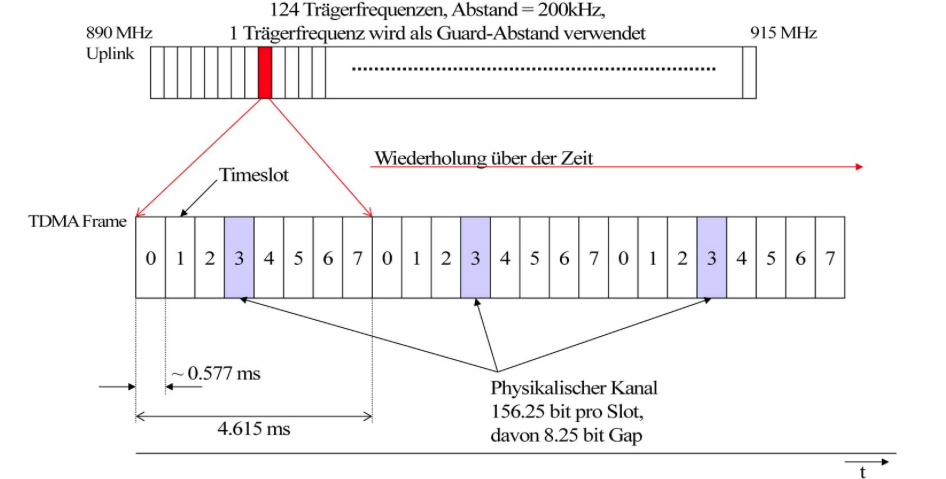
\includegraphics[width = 0.5 \linewidth]{./Pics/GSMRahmenstruktur}

\subsubsection{Mulitplextechniken Überblick}
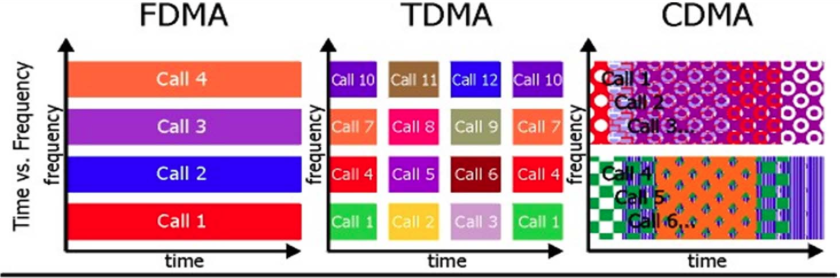
\includegraphics[width = 0.5 \linewidth]{./Pics/GSMMuxTechniken}

\begin{description}
	\item[FDMA] Frequency Division Multiple Access
	\begin{itemize}
		\item Verschieden Frequenzkanäle
		\item Pro Frequenz nur einer der Spricht
	\end{itemize}
	\item[TDMA] Time Division Muliple Access
	\begin{itemize}
		\item Verschieden Frequenzkanäle
		\item Mehrere Timeslots pro Frequenz
		\item Die Übertragungsrate wird auf mehrere Aufgeteilt
	\end{itemize}
	\item[CDMA] Code Division Multiple Access
	\begin{itemize}
		\item Verschieden Frequenzkanäle
		\item Jeder Spricht in einem eigenen Code gleichzeitig
		\item kann man sich anhand mehrere Leute in einem Raum die verschiedene Spachen sprechen vorstellen
	\end{itemize}
\end{description}

\subsection{Übertragungsprobleme}
\begin{minipage}{0.5 \linewidth}
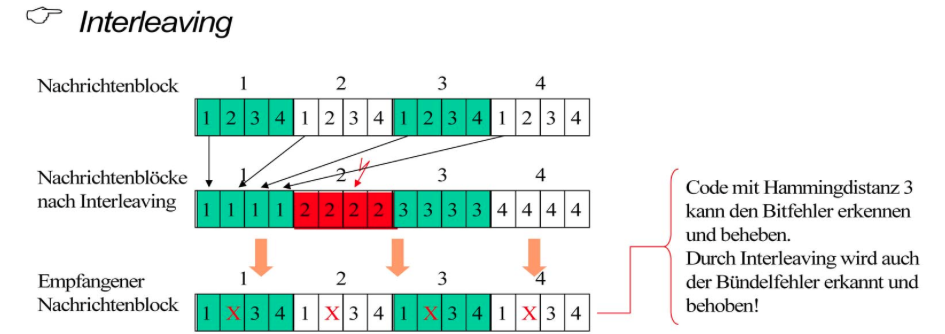
\includegraphics[width = \linewidth]{./Pics/GSMInterleaving}
\end{minipage}
\begin{minipage}{0.5 \linewidth}
\begin{itemize}
\item \textbf{Interleaving}
\item Auftretende Fehler sind meist Bündelfehler, d.h. ein ganzer Burst ist gestört
\item Es ist nicht möglich Codes mit mehr Kontrollstellen einzuführen, um so mehr Fehlerstellen zu korrigieren
\end{itemize}
\end{minipage}


\begin{minipage}{0.5 \linewidth}
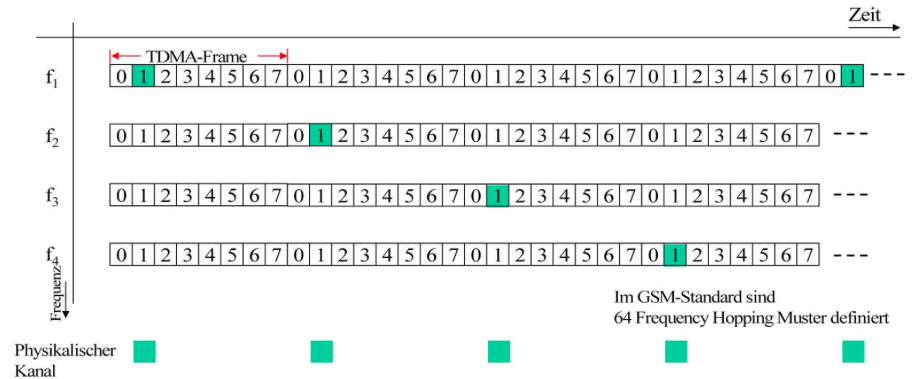
\includegraphics[width = \linewidth]{./Pics/GSMFreqHopping}
\end{minipage}
\begin{minipage}{0.5 \linewidth}
\begin{itemize}
\item \textbf{Rayleigh Fading} ist frequenzabhängig
\item Um bessere Übertragungsqualität zu erreichen, ist eine Bandspreiung sinnvoll
\item Durch \texttt{Frequency Hopping} wird eine Bandspreizung erreicht!
\end{itemize}
\end{minipage}

\subsubsection{Time Dispersion} 

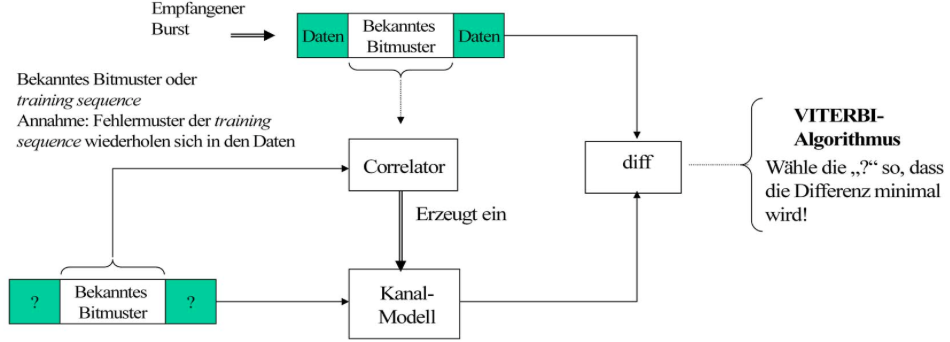
\includegraphics[width = 0.6\linewidth]{./Pics/GSMTimeDispersion}

\subsubsection{Rahmensynchronisation - Timing Advance}
\begin{itemize}
\item Timing Advance ist ein Lösungsansatz der speziell die Rahmensynchronisation vornimmt
\item Hierzu wird ein Protokoll definiert
\begin{itemize}
\item Messen der Laufzeit zwischen MS und BTS
\item Senden einer Korrekturzeit von der BSC via BTS an die MS, ob die MS früher oder später senden muss
\end{itemize}
\item Für die Anmeldeprozedur muss ein verkürzter Burst zur Verfügung gestellt werden
\end{itemize}

\subsubsection{Access Burst}
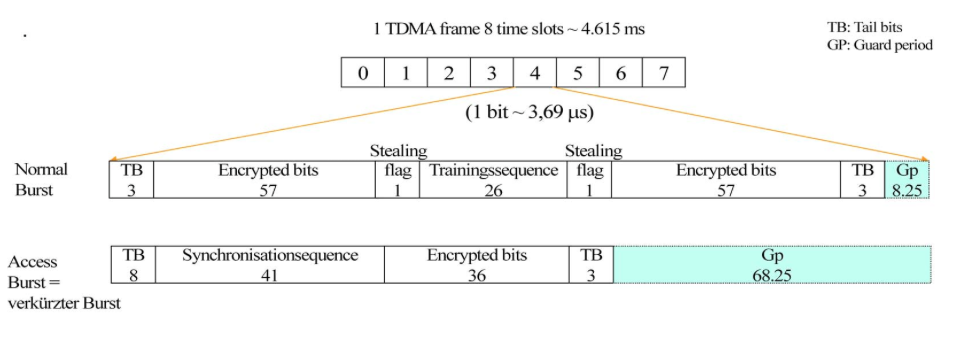
\includegraphics[width = 0.6\linewidth]{./Pics/GSMAccessBurst}

\subsection{Zusammenfassung GSM Übertragungsprozess}

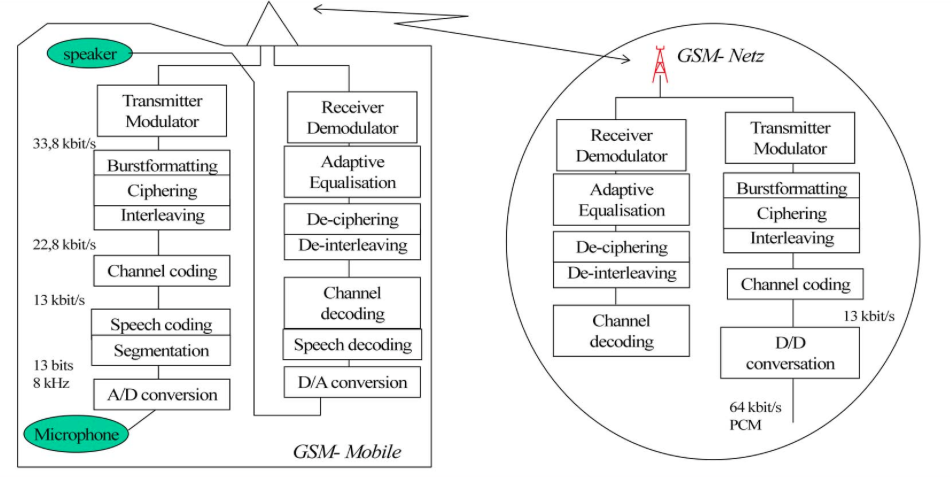
\includegraphics[width = 0.6\linewidth]{./Pics/GSMZusammenfassung}

\subsection{GSM Protokoll Stack}
\begin{minipage}{0.5 \linewidth}
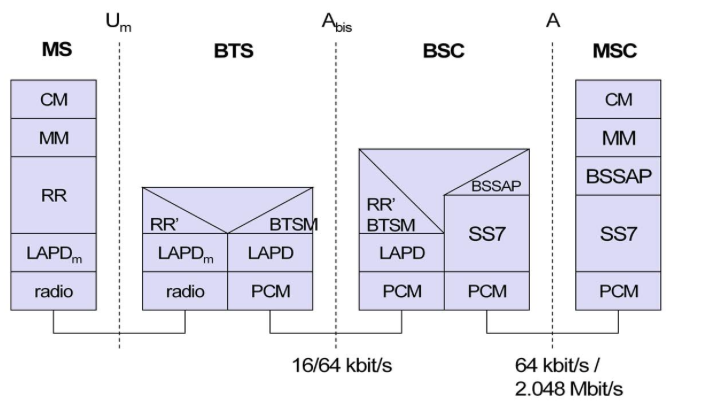
\includegraphics[width = \linewidth]{./Pics/GSMProtokollStack}
\end{minipage}
\begin{minipage}{0.5 \linewidth}
\begin{description}
\item[CM] Communication Management
\item[MM] Mobility Management
\item[RR] Radio Resource Management
\item[LAPD] Link Access Protocol for D-Channel
\item[BTSM] BTS Management
\item[BSSAP] Base Station System Application Part
\item[SS7] Signaling System No. 7
\end{description}
\end{minipage}

\subsection{Kanalstruktur}
\subsubsection{Übersicht}
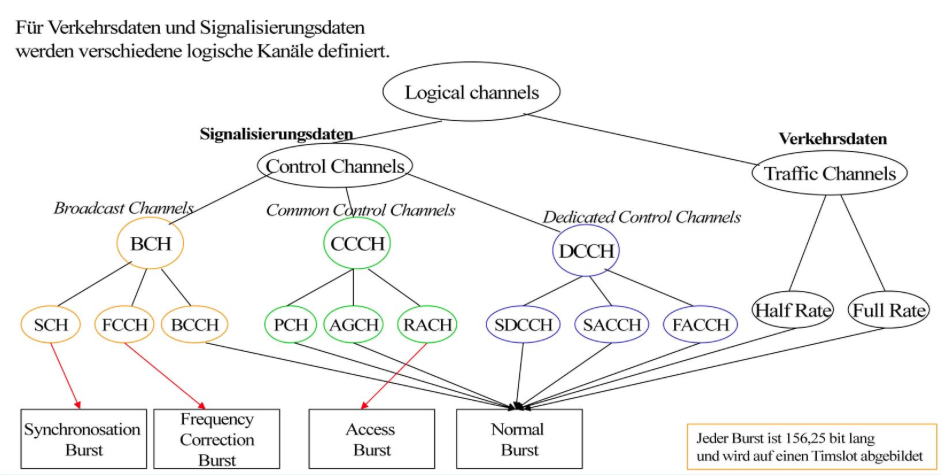
\includegraphics[width = 0.5 \linewidth]{./Pics/GSMKanalstruktur}

\subsubsection{Traffic Channels}
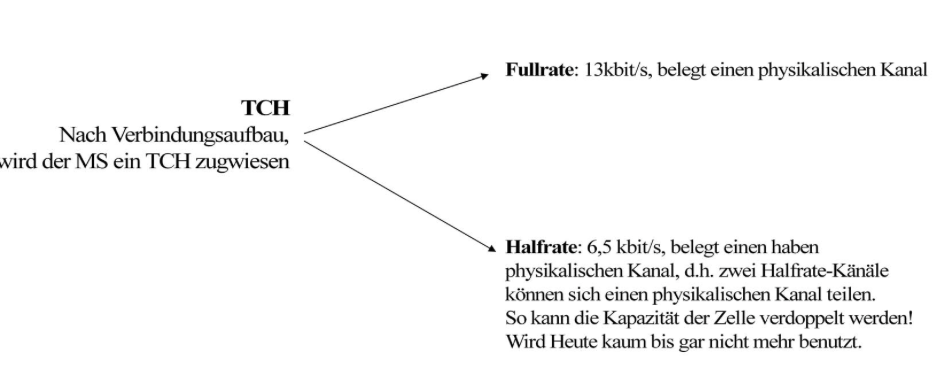
\includegraphics[width = 0.5 \linewidth]{./Pics/GSMTCH}
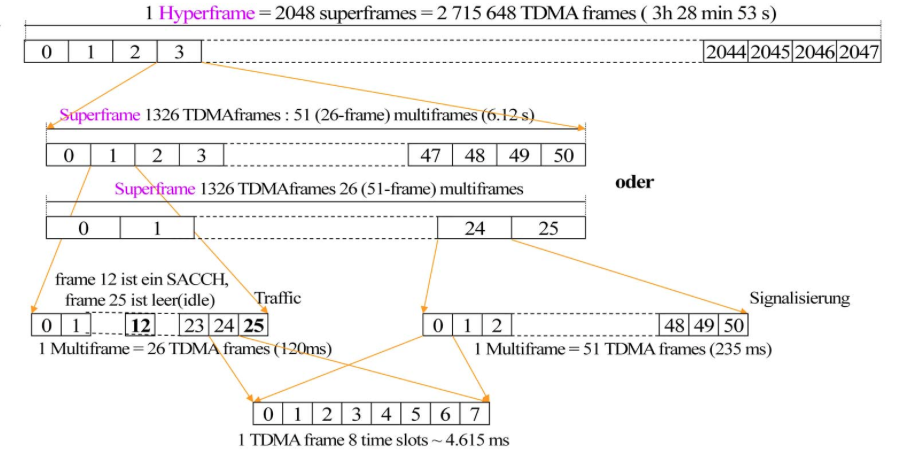
\includegraphics[width = 0.5 \linewidth]{./Pics/GSMFRrameBurstStruktur} $\;$\\ \\
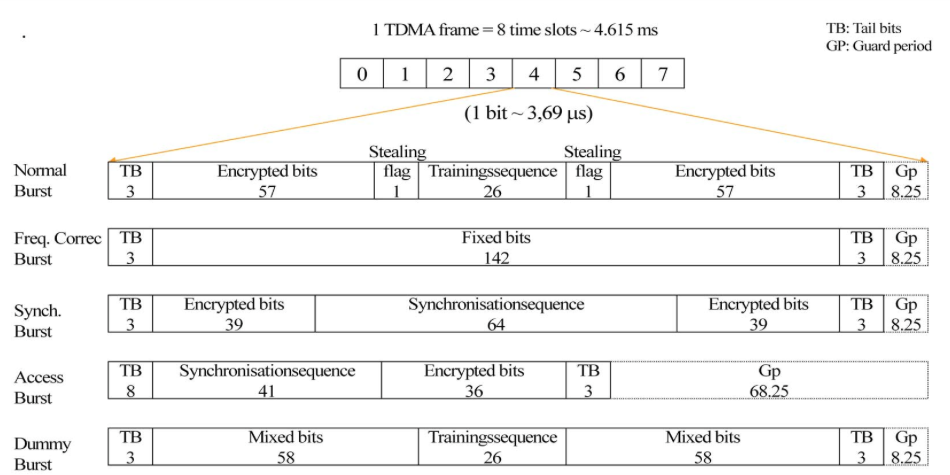
\includegraphics[width = 0.5 \linewidth]{./Pics/GSMBurstStruktur}
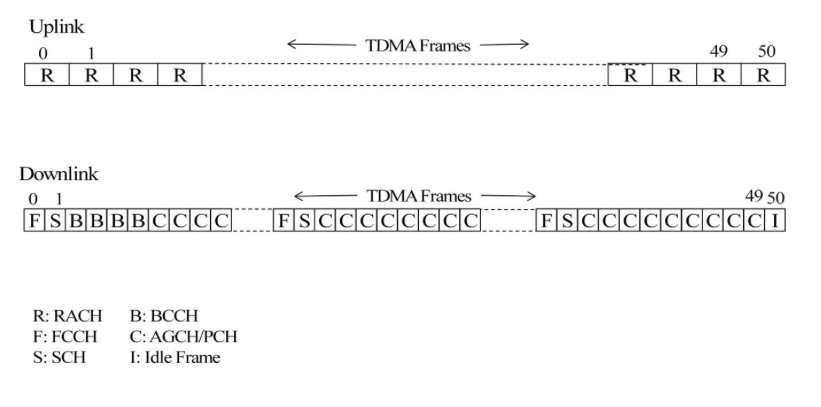
\includegraphics[width = 0.5 \linewidth]{./Pics/GSMMultiframe}
\subsubsection{Signalisierungsdaten}
\begin{tabular}{p{0.15 \linewidth} p{0.15 \linewidth} p{0.3 \linewidth} p{0.3 \linewidth}}
\toprule
Logischer Kanal & Richtung & BTS & MS \\
\midrule
AGCH & Downlink point to point & Weist der MS einen Signalisierungskanal (SDCCH) zu & Empfängt eine Signalisierungskanalzuweisung \\
\midrule
BCCH - Broadcast Control Channel & Downlink point to Multipoint & Verteilt allgemeine Zellinformationen, wie z.B. LAI (Local Area Identity), die BCCH Träger der Nachbarzellen, Max. Ausgangsleistung & Empfängt die LAI und leitet  ggf. ein Location update ein. 
Stellt die Ausgangsleistung ein.
 Erstellt eine List der Nachbarzell-BCCHs für die Leistungsmessungen der BCCH-Träger \\
\midrule
CBCH - Cell Broadcast Channel & Downlink point to multipoint & Dient zum versenden von Broadcast-Kurznachrichten & Empfang von Broadcast-Kurznachrichten\\
\midrule
FACCH Fast Associated Control Channel & Up- und Downlink point to point & Übermittelt Handover-Informationen & Übermittelt Handover-respons\\
\midrule
FCCH - Frequency Correction Channel & Downlink point to Multipoint & Überträgt die Trägerfrequenz & Identifiziert den BCC-Träger und synchronisiert auf der Frequenz \\
\midrule
PCH - Paging Channel & Downlink point to point & Signalisisert einen eingehenden Ruf oder ein SMS. Die Nachricht enthält die Identifikationsnummer des Mobilfunkkunden (IMSI) & Die MS hört regelmässig auf den PCH und reagiert, wenn die eigene Mobile Subscriber ID addressiert wird \\
\midrule
RACH - Random Access Channel & Uplink point to point & Empfängt die Anforderung einer MS einen Signalisierungskanal aufzubauen (SDCCH) & Eigentsändiger Verbindungsaufbau oder Antwort auf Request über den PCH \\
\midrule
SACCH Slow Associated Conrtol Channel & Up- und Downlink point to point & Erteilt Befehle zur Regelung der Sendeleistung und zum timing advance & Sendet durchschnittsmessungen der eigenen BTS (Signalstärke und Qualität) und der Nachbar BTSen (Signalstärke) \\
\midrule
SCH - Synchronisation Channel & Downlink point to Multipoint & Enthält Daten über die TDMA Rahmenstruktur in einer Zelle sowie die BTS - ID & Synchronisiert mit der Rahmenstruktur \\
\midrule
SDCCH - Standalone Dedicated Control Channel & Up- und Downlink point to point & Die BTS schaltet auf einen SDCCH.
Die Verbindungsaufbau Prozedur wird abgewickelt und ein TCH wird zugewiesen.
SDCCH wird auch zur Übermittlung von SMS verwendet & Die MS schaltet auf ein SDCCH.
Die Verbindungsaufbau-Prozedur wird abgewickelt und ein TCH wird zugewiesen (Träger und Slot).\\
\bottomrule

\end{tabular}

\subsection{MSISDN - Mobil Station/Subscriber Integrated Services Digital Network}

\begin{minipage}{0.6 \linewidth}
\begin{itemize}
\item Ordnet Mobiltelefonen eindeutige Nummern zu (Telefonnummer)
\item Die maximale Lände einer MSISDN beträgt 15 digits
\item ist die einzige Nummer, die der Subscriber kennt
\end{itemize}
\end{minipage}
\begin{minipage}{0.4 \linewidth}
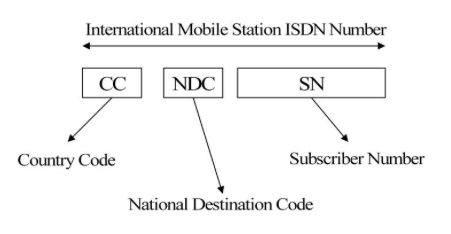
\includegraphics[width =  \linewidth]{./Pics/GSMMSISDN}
\end{minipage}

\begin{minipage}{0.6 \linewidth}
\begin{itemize}
\item IMSI - International Mobile Subscriber Identity
\begin{itemize}
\item Ist die eindeutige Identifikation eines Mobilfunk-Subscribers
\item Alle, zu einem Benutzer gehörenden Informationen, sind unter der IMSI zugreifbar. Ost quasi der Primary key vom HLR
\item Wird benutzt zur Signalisierung innerhalb des PLMN (Public Land Mobile Network)
\item Die IMSI ist gespeichert in der
\begin{itemize}
\item SIM Karte 
\item HLR
\item Serving VLR
\end{itemize}
\end{itemize}
\item TMSI - Temporary Mobile Subscriber Identity 
\begin{itemize}
\item Ist eine temporäre IMSI, die der MS während des Verbindungsaufbaus übergeben wird
\item Soll die Subscriberidentität an der Luftschnittstelle verschleiern
\item Die TMSI
\begin{itemize}
\item hat nur lokale Bedeutung (MSC/VLR Bereich)
\item Nicht grösser als 8 digits
\end{itemize}
\item Die TMSI ändert sich
\begin{itemize}
\item In bestimmten Intervallen
\item Bei einem Ereignis wie z.b. location update
\end{itemize}
\end{itemize}
\item MSRN - Mobile Station Roaming Number
\begin{itemize}
\item ist eine temporäre Nummer (gleicher Aufbau wie MSISDN), due während des Verbindungsaufbaus zu einem Subscriber in ein Netz vergen wird. Die MSRN wird durch das VLR vergeben und ist ebenfalls im HLR abgespeichert
\end{itemize}
\item LAI - Location Area Identity
\begin{itemize}
\item jede LA ist eindeutig durch eine LAI identifizierbar. Wird verwendet für:
\begin{itemize}
\item Paging
\item Location Updating
\end{itemize}
\item LAC - Location Area Code ein 16 Bit-feld zur Identifizierung verschiedener Location Areas in einem PLMN
\end{itemize}
\item CGI - Cell Global Identity
\begin{itemize}
\item Wird zur Identifizierung einer Zelle in einer Location Area benutzt
\end{itemize}
\item BSIC - Base Station Identity Code
\begin{itemize}
\item Dient den Mobilstationen zur Unterscheidung zwischen den benachbarten Basisstationen
\item besteht aus NCC (Network Color Code, 3 Bit) zur Identifizierung des PLMN und 
\item BCC (Basestation Color Code, 3 Bit) zur Unterscheidung der verschiedenen Nachbarzellen 
\end{itemize}
\end{itemize}
\end{minipage}
\begin{minipage}{0.4 \linewidth}
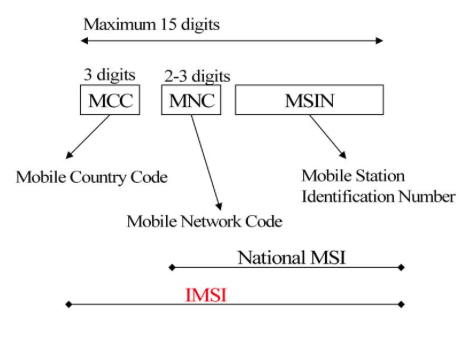
\includegraphics[width =  \linewidth]{./Pics/GSMITMSI} 
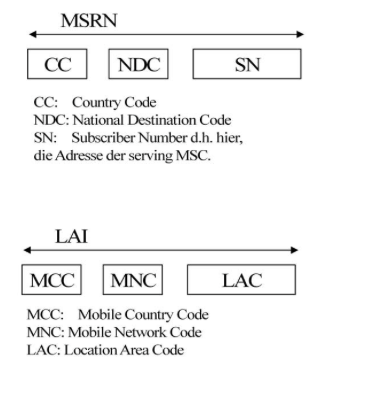
\includegraphics[width =  \linewidth]{./Pics/GSMMSRNUndLAI} 
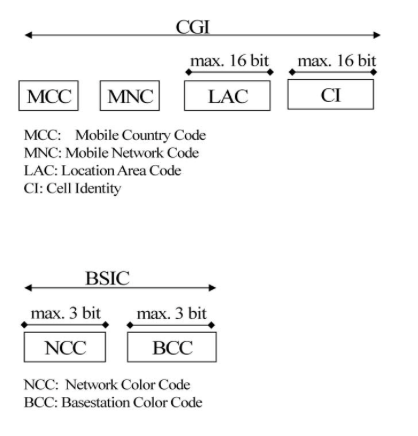
\includegraphics[width =  \linewidth]{./Pics/GSMCGIundBSIC} 
\end{minipage}

\subsection{Abläufe}
\subsubsection{Die Rolle der SIM}
Die SIM (Subscriber Identity Module) Karte ist die individuelle oder personalisierte Zugangsberechtigung zum PLMN.
\begin{itemize}
\item Die SIM Karte ist eine Chipkarte, die in eine MS eingefügt werden muss, um sich bei einem PLMN anzumelden
\item Die SIM speichert:
\begin{itemize}
\item Permanente Daten, z.B. IMSI, authentification key Ki, Liste der Trägerfrequenzen
\item Temporäre Daten, z.B. den aktuellen LAC, Zeitintervall für das location update, verbotene PLMNs....
\item Service-Daten, Service-Tabellen der zusätzlichen Dienstmerkmale, z.B. Spracheinstellungen, Taxiruf....
\end{itemize}
\item Es werden zwei Kartentypen unterschieden (gemäss Wikipedia 5)
\begin{itemize}
\item ID-1 SIM Card in Kreditkartengrösse (gemäss Wikipedia Standard SIM)
\item Plug-in SIM (kleiner als die ID-1) für semi-permanente Installation (gemäss Wikipedia Mini SIM)
\item seit 2003 Micro SIM, ist kleiner als Mini SIM (gemäss Wikipedia)
\item seit 2012 Nano SIM, ist kleiner als Micro SIM (gemäss Wikipedia)
\item in Zukunft Embedded SIM (gemäss Wikipedia)
\end{itemize}
\end{itemize}

\subsubsection{Sicherheitsprotokolle und die Rolle des AUC}

\begin{minipage}{0.5 \linewidth}
\begin{itemize}
\item Die Hauptaufgabe des AUC (Authentication Center) ist, die Informationen bereitzustellen, die das MSC/VLR benötigen um den Subscriber zu authentisieren und einen Schlüssel zur Verschlüsselung der Daten zu finden
\item Dazu erzeugt das AUC ein so genanntes Triplet
\begin{itemize}
\item RAND (Random Number)
\item SRES (Sigend Respons)
\item ein Schlüssel KC zur Verschlüsselung 
\end{itemize}
\item mit einer Anfrage werden 1,3 oder 5 Triplets erzeugt
\end{itemize}
\vspace{0.5 cm}
\textbf{Die Authentifizierung kann erfolgen bei}
\begin{itemize}
\item der Registrierung {attatching the Network}
\item jedem Verbindungsaufbau
\item jedem Location Updating
\item vor dem Start von Zusatzdiensten
\end{itemize}
\end{minipage}
\begin{minipage}{0.5 \linewidth}
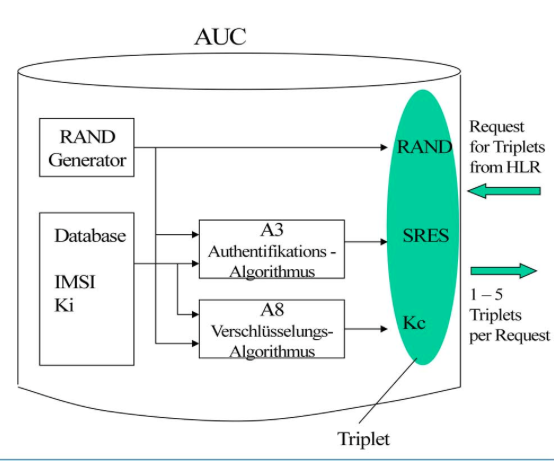
\includegraphics[width =  0.75 \linewidth]{./Pics/GSMAUC} 
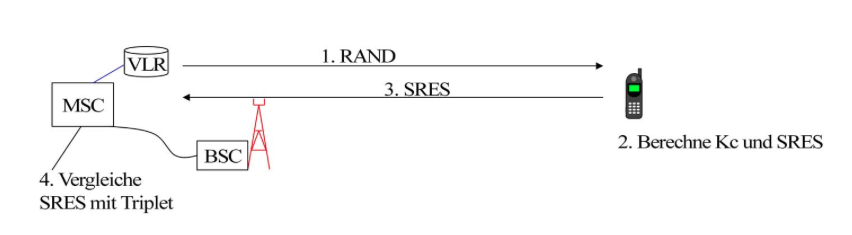
\includegraphics[width =  \linewidth]{./Pics/GSMAuthentifizierung} 
\end{minipage}
\subsubsection{Verschlüsselungsprozedur}
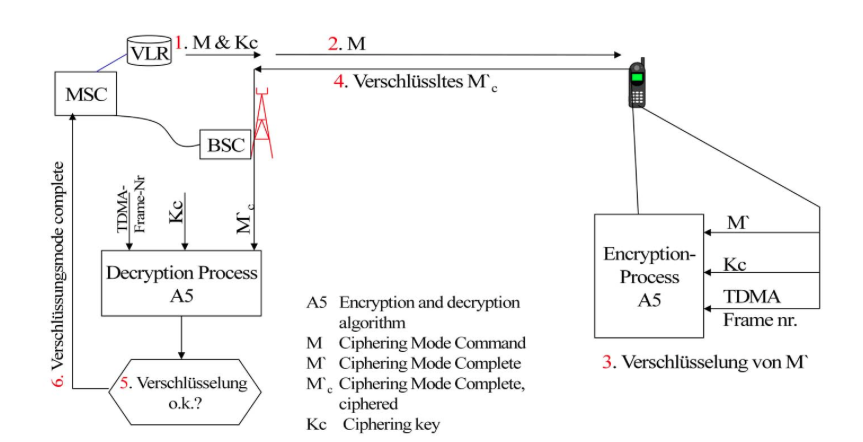
\includegraphics[width =  0.5 \linewidth]{./Pics/GSMVerschluesselung} 

\subsubsection{Anmeldeprozedur: IMSI Attach}
\begin{minipage}{0.5 \linewidth}
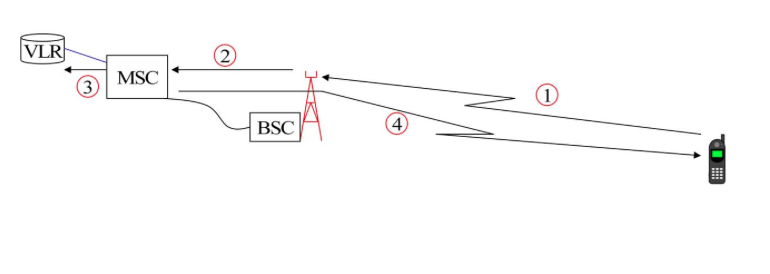
\includegraphics[width = \linewidth]{./Pics/GSMIMSIAttach}
\end{minipage}
\begin{minipage}{0.5 \linewidth}
\begin{enumerate}
\item Die MS sendet ein IMSI attach an das Netz mit der Zustandsangabe Idle.
\item Das VLR prüft, ob ein Datensatz der MS vorliegt. Liegt noch kein Datensatz vor, so kontaktiert das VLR das HLR und fordert die Subscriberinformation an. Hat sich ferner die LA geändert, so muss die neue LA ebenfalls ins VLR eingetragen werden
\item Das VLR setzt den Zustand der MS auf Idle
\item Es erfolgt eine Bestätigung an die MS, das die Anmeldung erfolgreich durchgeführt wurde.
\end{enumerate}
\end{minipage}

\subsubsection{Anmeldeprozedur: Location Update}
\begin{minipage}{0.5 \linewidth}
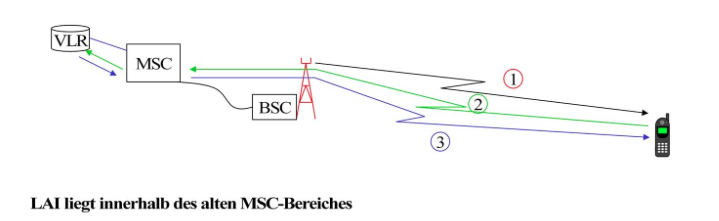
\includegraphics[width = \linewidth]{./Pics/GSMLocationUpdate}
\end{minipage}
\begin{minipage}{0.5 \linewidth}
\begin{enumerate}
\item Die MS hört ständig den aktuellen BCCH mit. Hier erhält sie unter anderem auch die Information über die LAI. Ist die LAI unterschiedlich der auf der SIM gespeicherten, so muss ein location update durchgeführt werden. 
\item Die MS muss dazu eine Verbindung zum Netz aufbauen (Anforderung eines SDCCH). Eine Authentisierung wird durchgeführt.
\item Ist die Authentisierung erfolgreich wird ein Location update Request an das System gesendet.
\item Hat kein MSC-Wechsel stattgefunden, so aktualisiert die aktuelle MSC den LAI im VLR und gibt den Signalisierungskanal wieder frei.
\end{enumerate}
\end{minipage}

\subsubsection{Abgehender Ruf}
\begin{minipage}{0.5 \linewidth}
\begin{enumerate}
\item Via RACH wird erst ein Signalisierungskanal angefordert
\item Die BSC teilt via AGCH der MS einen SDCCH zu
\item Die MS sendet eine set-up request an das MSC. Ferner werden die folgenden Prozeduren durchgeführt:
\begin{enumerate}
\item Die MS wird als aktiv im VLR eingetragen
\item Die Authentifizierungsprozedur wird durchgeführt
\item Die Verschlüsselung wird eingeschaltet
\item Die Ziel-Subscribernummer wird an das Netz übermittelt
\item Prüfen, ob abehender Rufe gesperrt sind
\end{enumerate}
\item Die MSC instruiert die BSC einen idle TCH zu reservieren. Ferner müssen sich die BTS und die MS auf den TCH synchronisieren
\item Die MSC leitet die Rufnummer weiter an die Zieladresse (ggf. PSTN)
\item Wenn der gerufene Teilnehmer antwortet werden die reservierten Kanäle geschaltet
\end{enumerate}
\end{minipage}
\begin{minipage}{0.5 \linewidth}
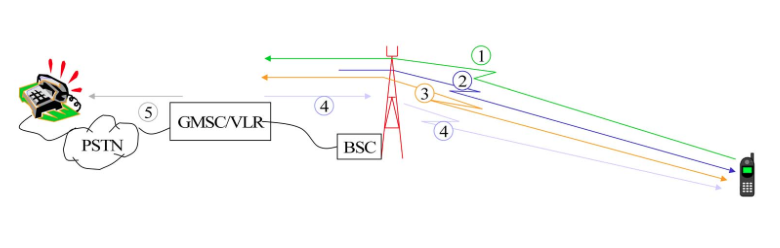
\includegraphics[width = \linewidth]{./Pics/GSMRuf}
\end{minipage}

\subsubsection{Ankommender Ruf}
\begin{minipage}{0.5 \linewidth}
Der Hauptunterschied zu einem abgehenden Ruf besteht darin, dass der Zielteilnehmer erst noch gesucht werden muss. Die MSISDN kann nicht unmittelbar für die Signalisierung genutzt werden. 

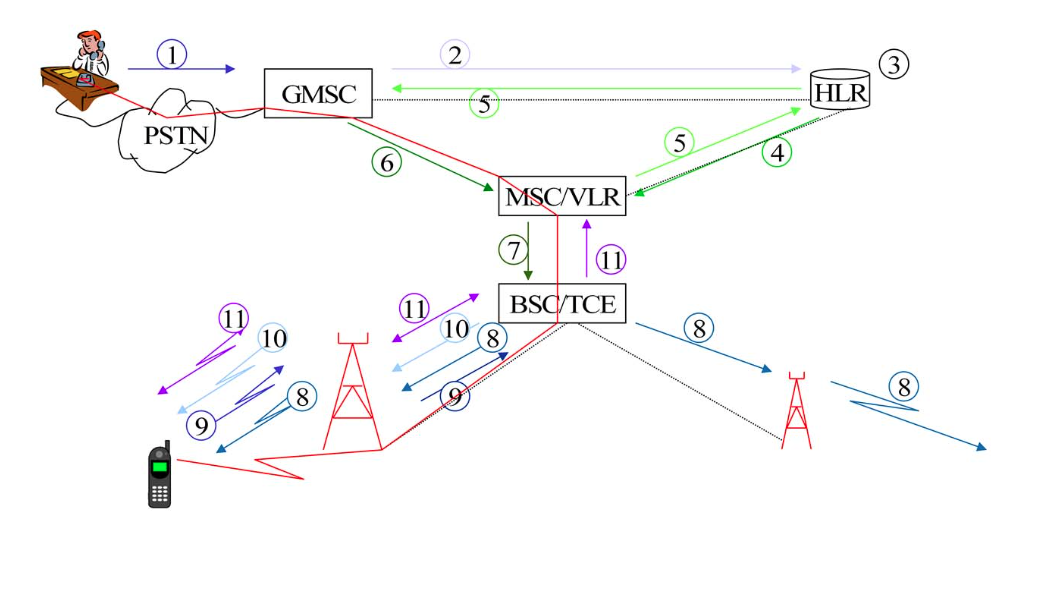
\includegraphics[width = \linewidth]{./Pics/GSMRuf2}
\end{minipage}
\begin{minipage}{0.5 \linewidth}
\begin{enumerate}
\item Die MSISDN wird im PSTN analysiert und an die GMSC weitergeleitet
\item Die GMSC des gerufen PLMN analysiert die MSISDN und fragt das HLR ab, zu welcher Serving MSC das Gespräch weitergeleitet werden muss. 
\item Das HLR überführt die MSISDN in die IMSI und entscheidet die Ziel MSC/VLR. Auserdem wird geprüft, ob zur Zeit Anrufe weitergeleitet werden sollen oder nicht
\item Das HLR fordert einen MSRN von der serving MSC/VLR an
\item Die serving MSC sendet via HLR die MSRN an die GMSC
\item Die GMSC wertet die MSRN aus und leitet den Ruf weiter
\item Die MSC/VLR kennt die LA und eine Paging-Nachricht wird an das BSC weitergeleitet
\item Die BSC leitet die Paging-Nachricht weiter an die BTSen der LA. Zur Identifikation dienen IMSI oder TMSI
\item Die MS antwortet mit einem request für einen SDCCH
\item Die BSC weist einen SDCCH über einen AGCH zu 
\item Die Call-set-up Prozedur wird durchgeführt und ein TCH reserviert sowie der SDCCH freigegeben
\item Die MS Signalisiert (ringing). Wird der Anruf angenommen wird durchgeschaltet
\end{enumerate}
\end{minipage}

\subsubsection{Handover}
\begin{minipage}{0.5 \linewidth}
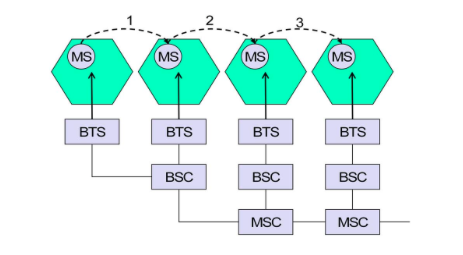
\includegraphics[width = \linewidth]{./Pics/GSMHandover}
\end{minipage}
\begin{minipage}{0.5 \linewidth}
\begin{enumerate}
\item Intra BSC Handover. BSC ist involviert.
\item BSC/Intra MSC Handover. Die BSC wird gewechselt. MSC ist involviert.
\item Inter MSC Handover. MSC wird gewechselt. Die alte MSC wird anchor MSC genannt, die neue MSC dann serving MSC nachdem der Handover abgeschossen ist. Das Billing (Verrechnung) wird jedoch immer von der anchor MSC gemacht. Das bedeutet, dass der Traffic immer von der serving MSC zur anchor MSC (uplink) und von der anchor MSC zur serving MSC (downlink) geleitet wird.
\end{enumerate}
\end{minipage}
\begin{minipage}{0.5 \linewidth}
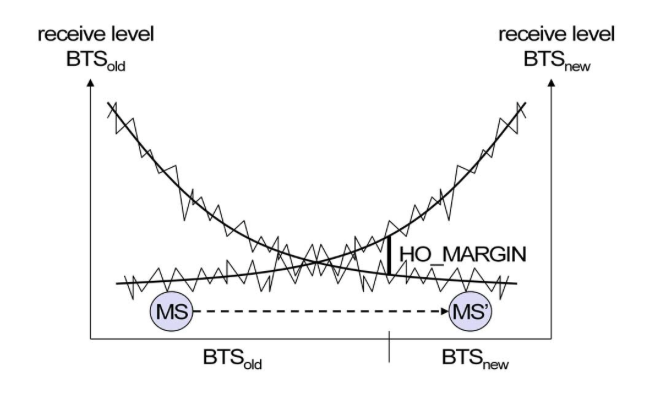
\includegraphics[width = \linewidth]{./Pics/GSMHandover2}
\end{minipage}
\begin{minipage}{0.5 \linewidth}
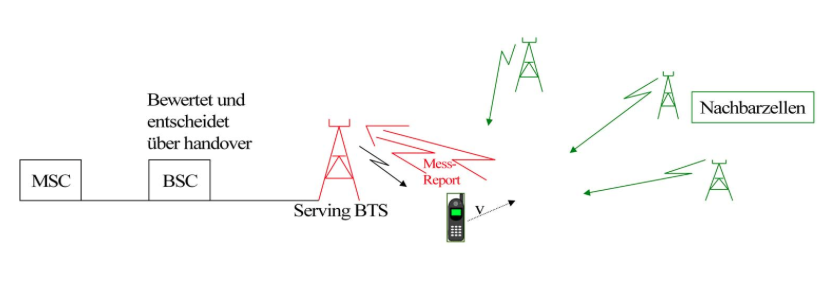
\includegraphics[width = \linewidth]{./Pics/GSMHandover3}
\end{minipage}

\begin{minipage}{0.5 \linewidth}
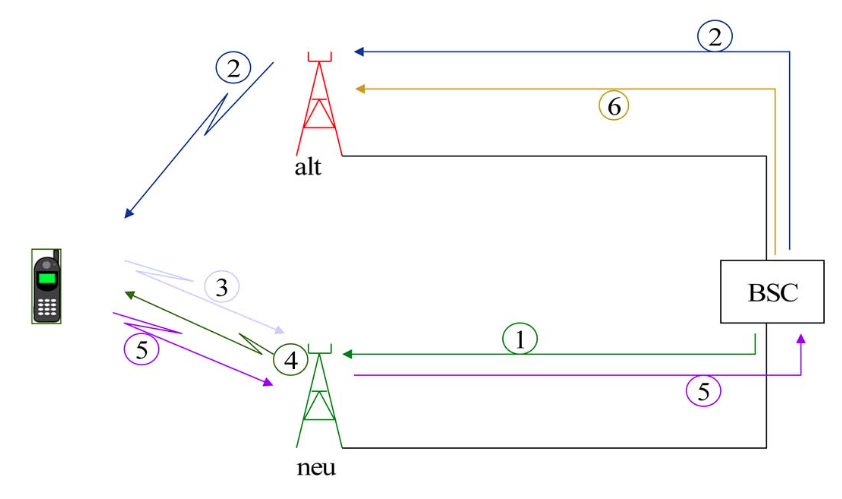
\includegraphics[width = \linewidth]{./Pics/GSMIntraHO}
\end{minipage}
\begin{minipage}{0.5 \linewidth}
\begin{enumerate}
\item Die BSC reserviert einen TCH in der neuen BTS
\item Die MS wird über die alte Verbindung (FACCH) über die neue Frequenz, den Time Slot und die Sendeleistung informiert
\item Die MS synchronisiert auf die Frequenz, die Rahmenstruktur und überträgt einen Handover Request über den FACCH. Der Handover Request hat nur einen Grösse von 8 Bit
\item Die BTS sendet die TA Information via FACCH
\item Die MS sendet ein Handover complete zur BSC über die neue BTS
\item Die alte BTS wird aufgefordert den TCH freizugeben, die Verbindung wird durchgeschaltet
\end{enumerate}
\end{minipage}

\begin{minipage}{0.5 \linewidth}
\begin{enumerate}
\item Die serving BSC sendet ein Handover Request an die MSC/VLR mit der ID der Zielzelle
\item Die MSC/VLR identifiziert die neue BSC und sendet ein Handover Request an die neue BSC
\item Die neue BSC reserviert einen TCH
\item Die BSC sendet eine Message via MSC und alte BSC an die MS
\item MS synchronisiert mit der neuen Frequenz auf neuem Timeslot und sendet Handover Request
\item Information über die TA wird übertragen
\item Die MS sendet Handover complete
\item Die MS sendet der alten BSC die Aufforderung den alten TCH freizugeben
\item Der alte TCH wird freigegeben. Die Verbindung ist durchgeschaltet 
\end{enumerate}
\end{minipage}
\begin{minipage}{0.5 \linewidth}
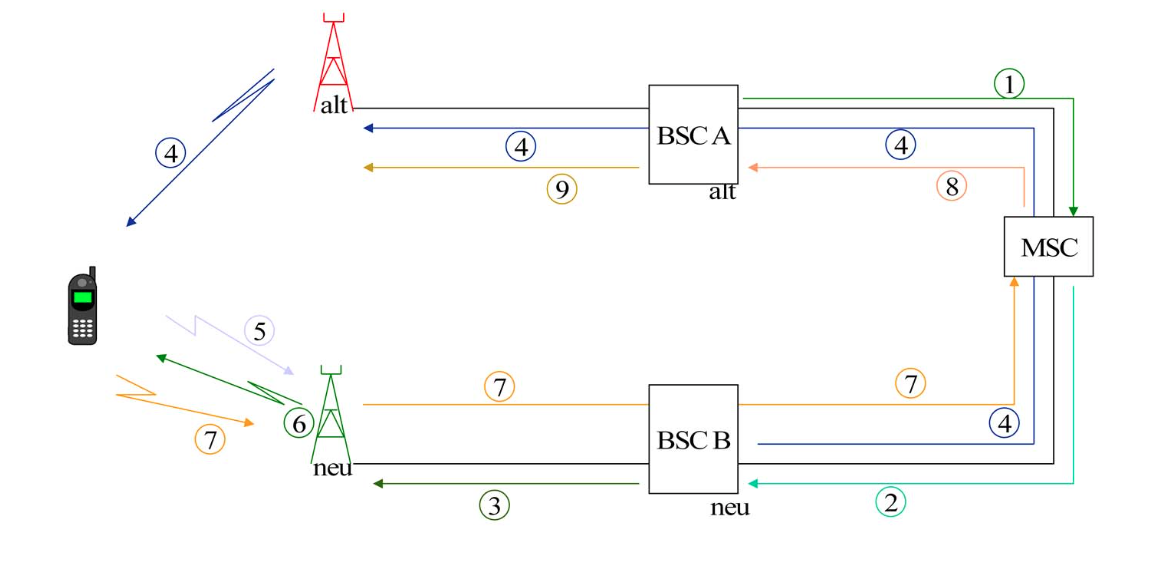
\includegraphics[width = \linewidth]{./Pics/GSMInterHO}
\end{minipage}

\begin{minipage}{0.5 \linewidth}
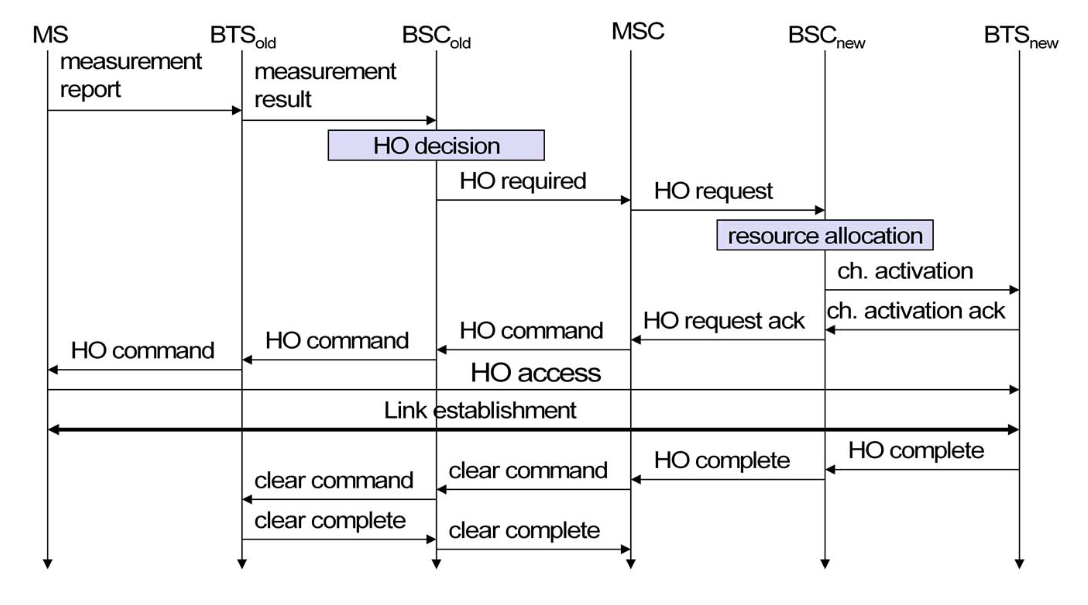
\includegraphics[width = \linewidth]{./Pics/GSMInterMSCHO}
\end{minipage}
\begin{minipage}{0.5 \linewidth}
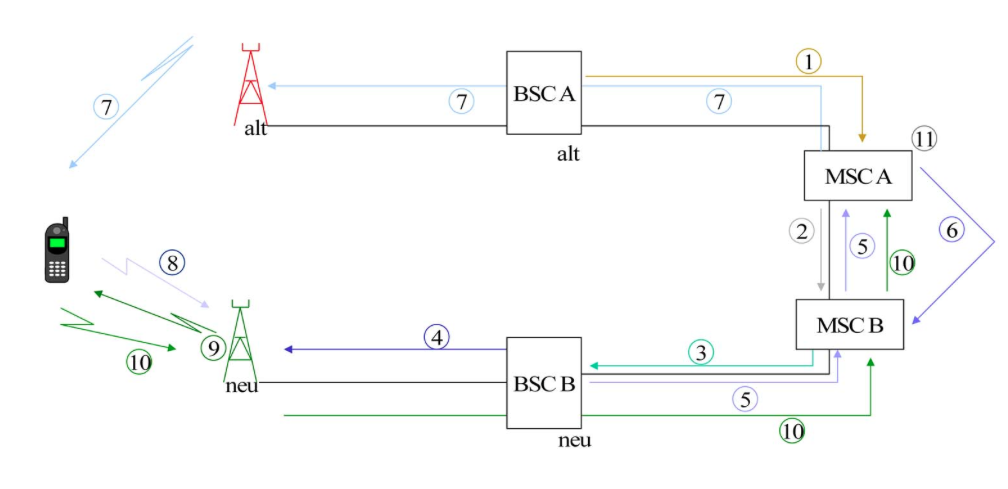
\includegraphics[width = \linewidth]{./Pics/GSMInterMSCHO2}
\end{minipage}

\begin{enumerate}
\item Die serving BSC sendet ein Handover Request an die MSC/VLR mit der ID der Zielzelle
\item Die MSC/VLR identifiziert die neue Zelle in einer anderen MSC und sendet ein help request an die neue MSC
\item Die neue MSC alloziert eine Handover-Number um den Ruf neu zu schalten. Ein Handover Request wird an die neue BSC gesendet
\item Die neue BSC reserviert einen TCH in der neuen Zelle
\item Die neuen BSC sendet eine Message (Zellinfo und Handover-Nummer) via MSCs und alte BSC an die MS
\item Es wird eine Verbindung zur neuen MSC geschaltet
\item Die MSC A sendet das Handover Command an die MS
\item Ms synchronisiert mit der neuen Frequenz auf neuem Timeslot und sendet Handover Request 
\item Information über die TA wird übertragen
\item Die MS sendet Handover Complete
\item Ein neuer Weg wird in der aletn MSC geschaltet und die Verbindung wird geschaltet
\item Die MSC sendet der alten BSC die Aufforderung den alten TCH freizugeben (nicht mehr im Bild eingetragen). Die Verbindung ist durchgeschaltet. 
\end{enumerate}
Die alte Msc behält die Hauptkontrolle über die Verbindung, bis sie ausgelöst wird.

\subsubsection{Roaming}
\begin{itemize}
\item Der prinzipielle Ablauf ist dem Anmelden im eigenen Netz identisch
\item Erst versucht die MS sich im eigenen Netz anzumelden, ist dies nicht möglich sucht es andere BCCH-Träger von fremden Netzen
\item Dann vergleicht es die gefundenen Netzte mit der Liste der verbotenen PLMNs (Auf SIM gespeichert)
\item Findet die MS ein geeignetes Netz, so läuft die Anmeldeprozedur wie vorher besprochen, nur dass das HLR des eigenen Netzes konsultiert wird
\end{itemize}

\subsubsection{HSCSD - High Speed Circuit Switched Data}
\begin{itemize}
\item Herkömmlich Datenübertragung ist standardisiert mit 9.6 kbit/s
\begin{itemize}
\item Gesicherte Datenübertragung geht runter bis auf 4.8 kbit/s
\item So genanntes advanced coding erlaubt 14.4 kbit/s
\end{itemize}
HSCSD High Speed Circuit Switched Data
\begin{itemize}
\item ist standardisiert
\item Bündelung von bis zu 4 TDMA-Slots, um eine höhere Datenrate zu erreichen. (AIUR Air Interface User Rate)
\item Vorteile:
\begin{itemize}
\item Verfügbar
\item Konstante Qualität
\item Einfach
\end{itemize}
\item Nachteile:
\begin{itemize}
\item Kanäle blockiert
\item Teuer für den Benutzer
\end{itemize}
\end{itemize}
\end{itemize}


\subsection{GPRS - General Packet Radio Service}
\subsubsection{Überblick}
\begin{itemize}
\item Datnepaket-Dienst
\item Dynamische Bündelung freier Slots zu hochbitratigen Datenkanälen, je nach coding Schema 8 bis 21.4 kbit/s
\item asymetrische Übertragung - Slots werden nur belegt, wenn effektiv übertragen wird
\item Gebühren nach Datenmenge und nicht mehr nach Zeit
\item Standartisierung 1998, Einführung 2001/2002
\item Erweiterung der bisherigen Netztopologie
\item geplant ist ein komplementärer Einsatz von GSM/GPRS und UMTS
\item Harmonisierung Internet und Mobilnetz dank IP
\end{itemize}
\subsubsection{GPRS Netzelemente}
\begin{itemize}
\item GSN: GPRS Support Nodes
\begin{itemize}
\item GGSN Gateway GSN - Gateway zu PDNs(Public Data Network)
\item SGSN Serving GSN - unterstützt die MS(location, billing security)
\end{itemize}
\item GR: GPRS Register - eine Ergänzung zum HLR zur Adressverwaltung
\item PCU Packet Control Unit - Übernimmt BSC Funktion im paketorientierten Netzwerk
\end{itemize}

\subsubsection{Architektur Übersicht}
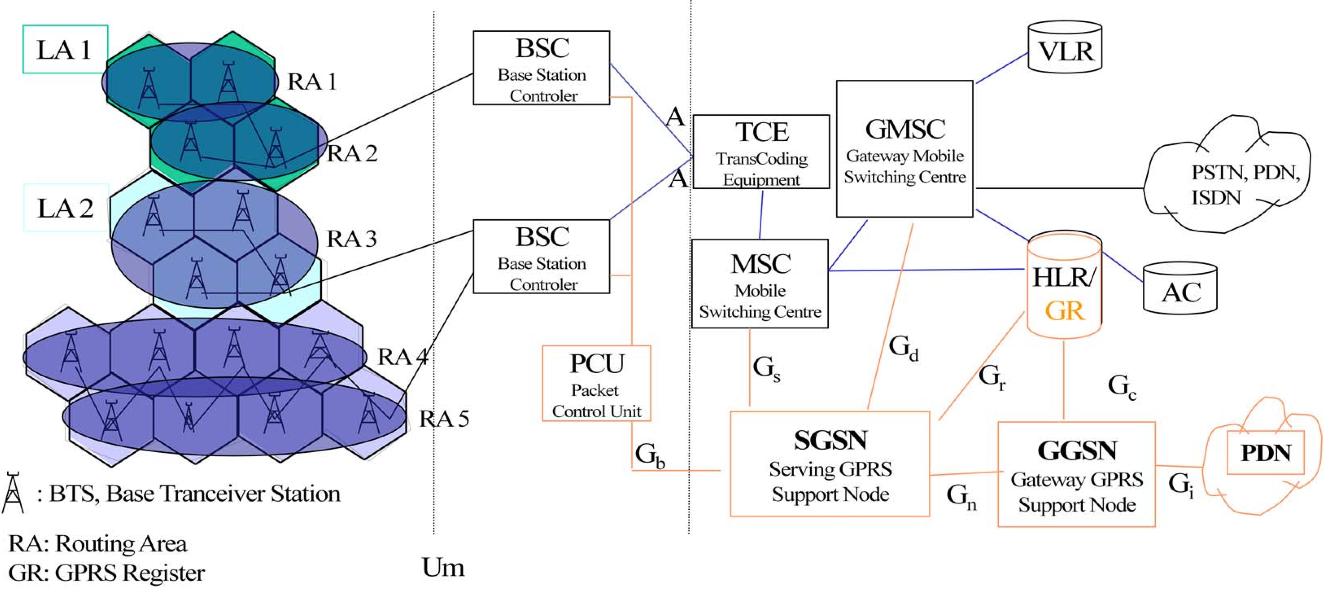
\includegraphics[width = \linewidth]{./Pics/GPRS.png} \\
Diese Grafik zeigt sehr gut, dass das GPRS kein neues Netz ist sondern eine Erweiterung von GSM. Orange eingefärbt sieht man die neuen Element. Man hat nun neben dem Verbindungsorientierten GSM Netz noch ein Paketorierntiertes GPRS Datennetz. Dieses Netz wird ausschliesslich zur Datenübertragung verwendet und kann wegen einer sehr hohen latenzzeit (bis 500ms) auch nicht für VOIP verwendet werden.

\subsubsection{Protocol stack}
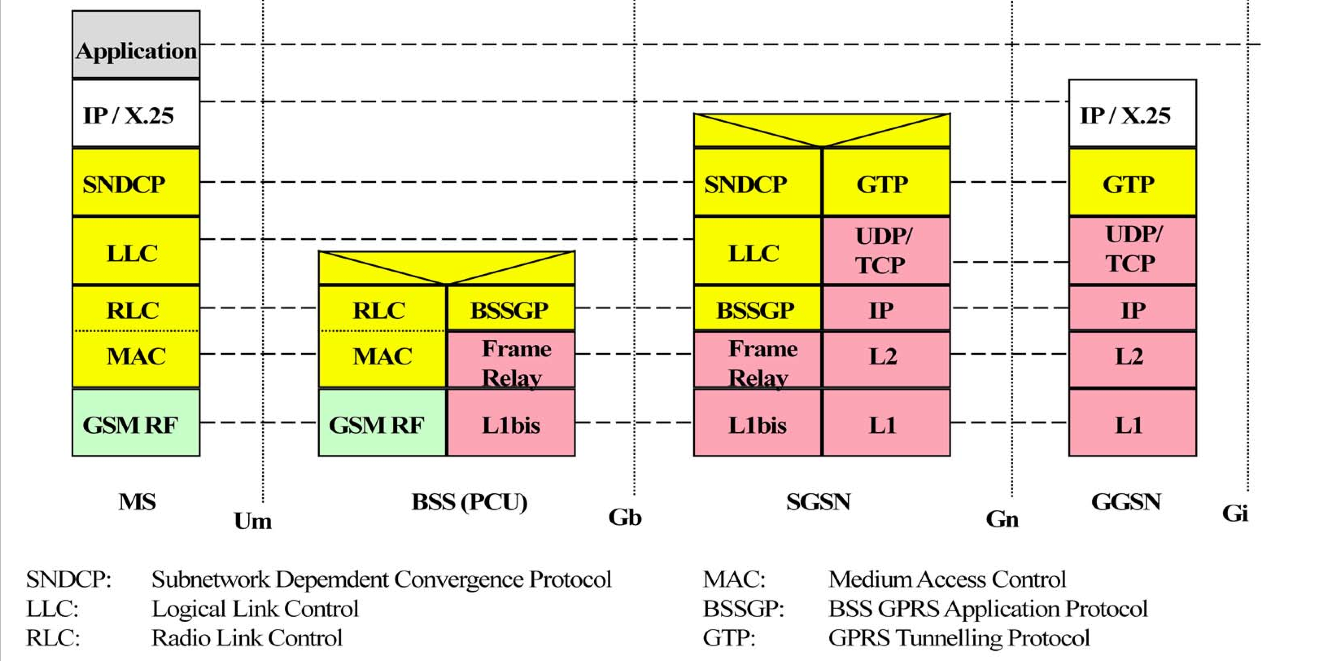
\includegraphics[width = \linewidth]{./Pics/GPRS2.png}

\begin{tabular}{|l|l|l|l|}
\hline
IP & Internet Protocol & X.25 & vorläufer von IP \\
SNDCP & Subnetwork Dependent Convergence Protocol & LLC & Logical Link Control \\
RLC  & Radio Link Control  & MAC & Medium Access Control \\
GSM RF &  Global System for Mobile Communications Radio Frequencies & BSSGP & Base Station System GPRS Protocol \\
GTP & GPRS Tunnelling Protocol & UDP & User Datagram Protocol \\
TCP & Transmission Control Protocol & & \\ 
\hline
\end{tabular}
\subsubsection{GTP}
Das GPRS Tunnelling Protocol baut IP-basierte Verbindungen durch den Backbone auf. Datenpakete werden eingepackt \& unter Benutzung des GTP getunnelt. GTP nutzt unterhalb TCP oder UDP  abhängig von der Nutzeranforderung. Das ganze GPRS Netzwerk basiert auf einem IP Hop, was das Routing im Backbone bei Mobilität vereinfacht.



\subsection{MPS - Mobile Positioning System}

\subsubsection{Verwendung}
\begin{description}
\item [MPS] Mobil Position Services
\item [Legal interception] Verfolgung von und Zugriff auf Zielpersonen durch die Polizei
\item [Desaster and Emergency Management] Suche nach vermissten und/oder hilflosen Personen
\end{description}
\vspace{0.5cm}

\begin{itemize}
\item Forderung durch Standards
\begin{itemize}
\item NG911(Next Generator 911): Suchradius < 10 m in 95 \% der Suchfälle
\end{itemize}
\item Hauptproblem
\begin{itemize}
\item Unterscheidung Nah- und Fernbereich
\item In Urbanen Regionen mit Häuserschluchten (Abdeckungen/Reflexionen)
\end{itemize}
\end{itemize}

\subsubsection{Verfahren zur Positionsbestimmung: Überblick}

\begin{minipage}{0.7 \linewidth}
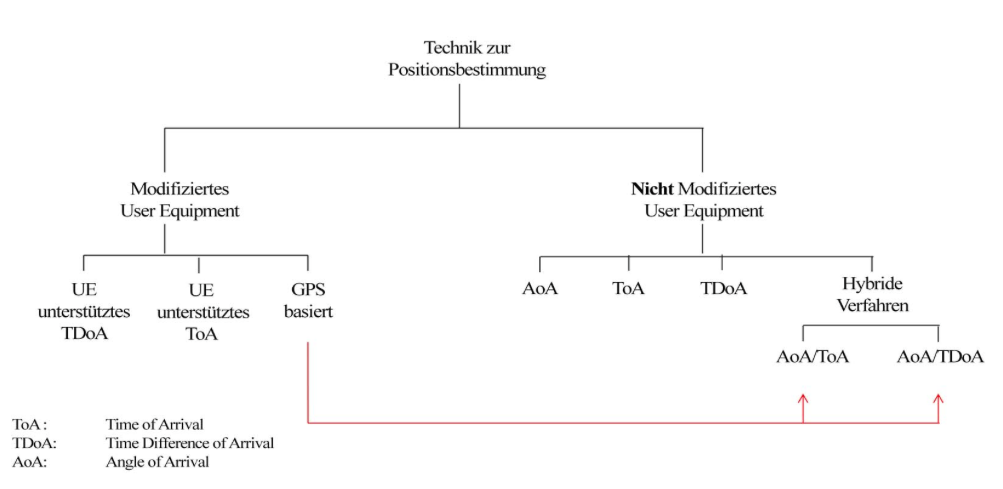
\includegraphics[width =\linewidth]{./Pics/MPS}
\end{minipage}
\begin{minipage}{0.3 \linewidth}
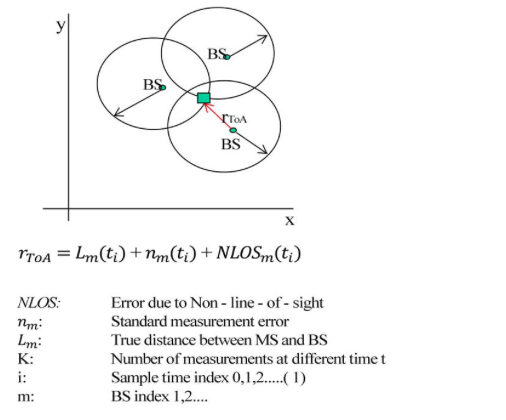
\includegraphics[width = \linewidth]{./Pics/TDoA}
\end{minipage}

TDoA oder hyperbolig PL Technique ist eine Verfeinerung der ToA und basiert auf einer zeitsynchronisierten (GPS) Location Measurement Units (LMUs) der Base Station.

Die LMUs wertet jeden UPLinkCall eines Subscribers aus. 

Das heute implementierte System bringt eine Genauigkeit kleiner 50m, benötigt werden aber eine freie Sicht zu mindestens 3 BS, je mehr desto besser. 

\subsubsection{Gegenstand der Forschung}
\begin{itemize}
\item Kombination von Mobilnetz und anderen RF Systemen Wi-Fi
\item Fehler Optimierung der ToA/TDoA Technologien
\item AoA Techniken, Probleme der Winkelbestimmung, Herausforderung an die Elektrotechnik - Antennen mit synthetischer Apertur
\item Phasenanalyse des Trägers, Probleme bei langsamen Mobilstationen (kein Dopplereffekt)
\item Auswertung typischer Netzwerkeigenschaften
\begin{itemize}
\item Messreports, Cell ID, Signal Fingerprints
\item Nachteil: der provider muss Daten vorhalten
\end{itemize}
\item Kombination von GPS(Empfang von nur einem Satelliten zur Zeitsynchronisation) mit ToA Phasenanalyse
\end{itemize}
\section{UMTS - Universal Mobile Telecommunications System}
\begin{minipage}{0.5\linewidth}
\subsection{UMTS Ziele}
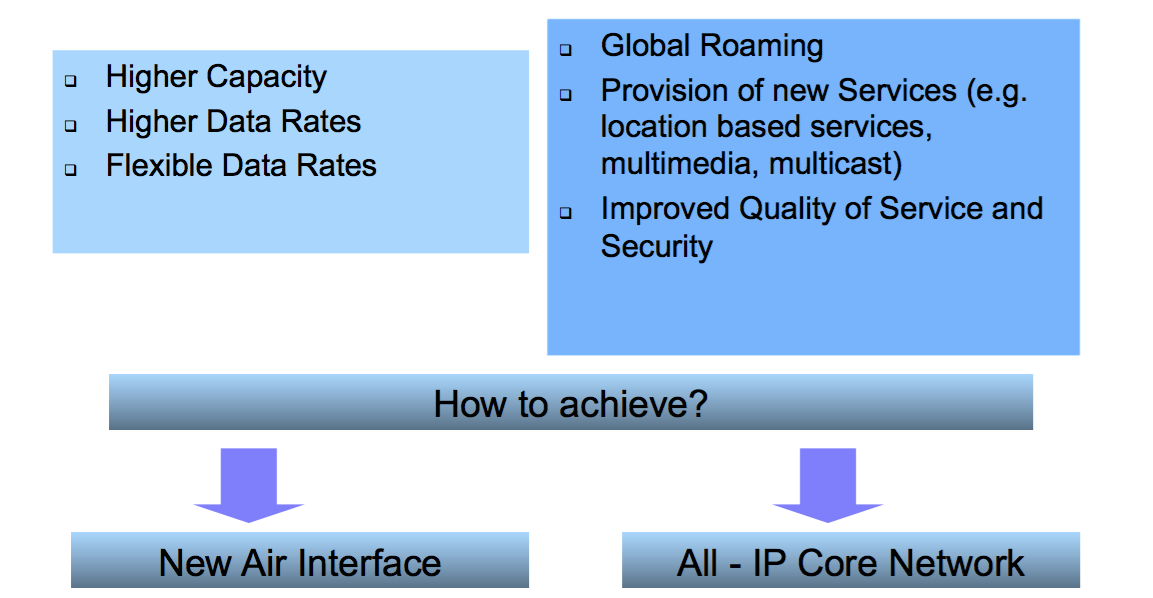
\includegraphics[width = \linewidth]{./Pics/UMTS}
\end{minipage}
\begin{minipage}{0.5\linewidth}
\subsection{UMTS Entscheidungfaktoren}
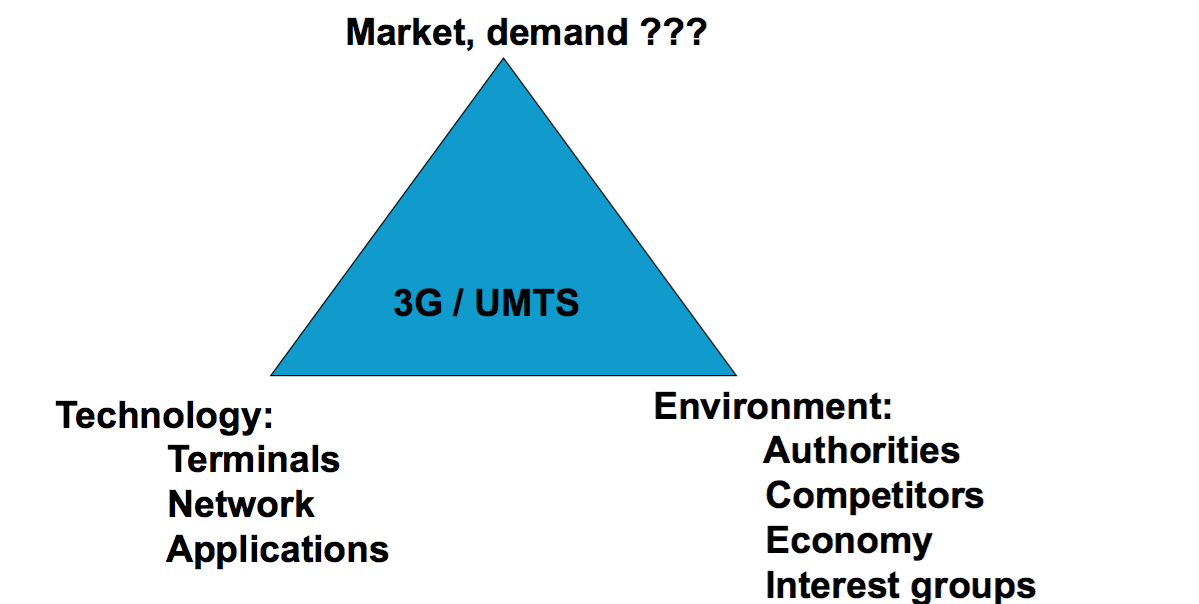
\includegraphics[width = \linewidth]{./Pics/UMTS3}
\end{minipage}

\begin{minipage}{0.5\linewidth}
\subsection{UMTS Verspricht}
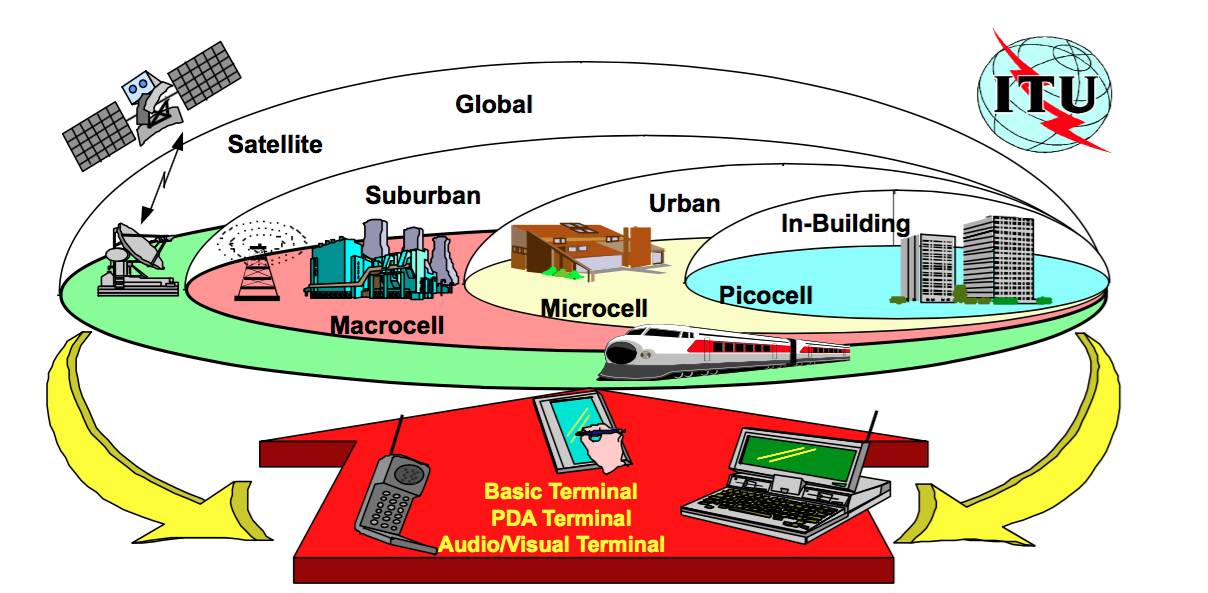
\includegraphics[width = \linewidth]{./Pics/UMTS2}
\end{minipage}
\begin{minipage}{0.5\linewidth}
\subsection{UMTS Klärende Fragen}
\begin{itemize}
\item Welche Netzelemente sind erforderlich ? 
\begin{itemize}
\item System Architecture
\item System Components and Identifiers
\end{itemize}
\item Wie Kommunizieren die Netzelemente ?
\begin{itemize}
\item Protocols and Logical Channels
\end{itemize}
\item Was sind die erforderlichen Netzprozeduren ? 
\begin{itemize}
\item Establish, Maintain and Release Communication Links
\item Provide sufficient Quality of Service
\end{itemize}
\item Wie wird der erforderliche QoS sichergestellt?
\begin{itemize}
\item Radio Access Network Design (im speziellen PHY)
\end{itemize}
\end{itemize}
\end{minipage}

\subsection{Evolution von GPRS zu UMTS}
\begin{minipage}{0.45\linewidth}
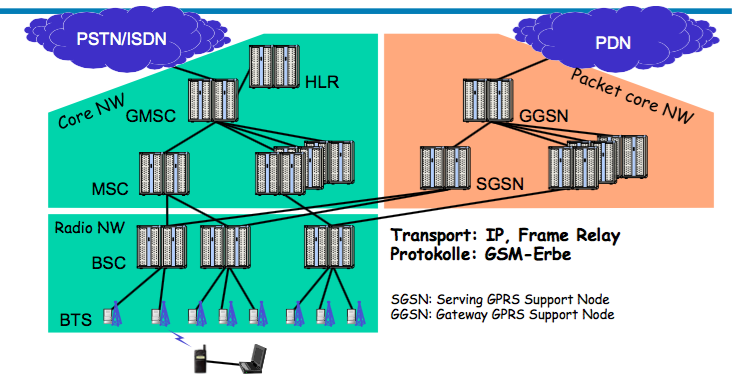
\includegraphics[width = \linewidth]{./Pics/UMTS4}
\end{minipage}
\begin{minipage}{0.1\linewidth}
$\Rightarrow$
\end{minipage}
\begin{minipage}{0.45\linewidth}
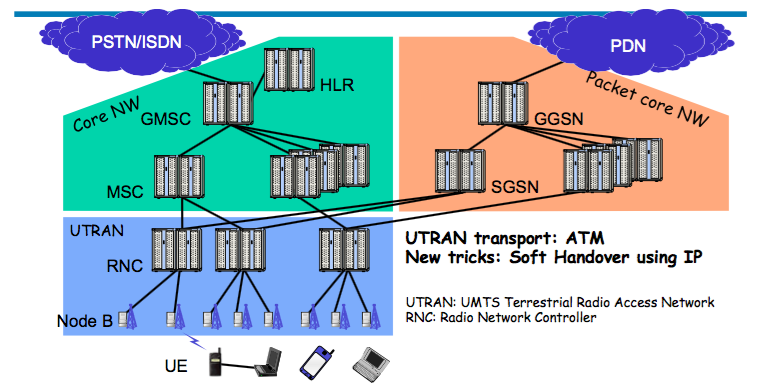
\includegraphics[width = \linewidth]{./Pics/UMTS5}
\end{minipage}

\subsection{UMTS Architektur}
\begin{minipage}{0.5\linewidth}
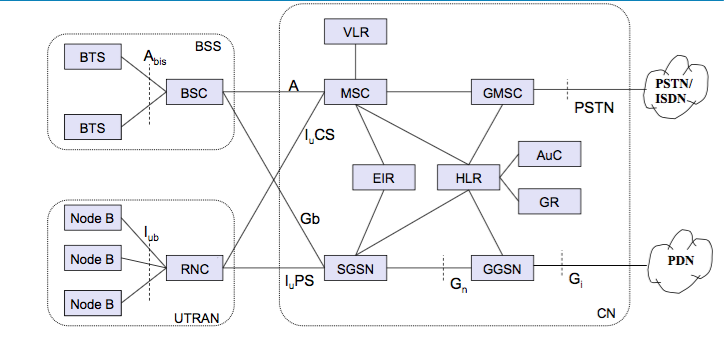
\includegraphics[width = \linewidth]{./Pics/UMTSArch} \\
\includegraphics[width = \linewidth]{./Pics/UMTSArch3}
\end{minipage}
\begin{minipage}{0.5\linewidth}
\begin{itemize}
\item Das Core Network (CN) und auch das Interface $I_u$ sind aufgeteilt in zwei logische Domänen:
\item Circuit Switched Domain (CSD)
\begin{itemize}
\item Circuit Switched Dienst inkl. Signalisation
\item Ressourcen -Reservation beim Verbindungsaufbau
\item GSM Komponenten (MSC, GMSC, VLR)
\item $I_uCS$
\end{itemize}
\item Packet Swiched Domain (PSD)
\begin{itemize}
\item GPRS Komponenten (SGSN, GGSN)
\item $I_uPS$
\end{itemize}
\item Release 99 benutzt das GSM/GPRS Netzwerk und ergänzt das Netzwerk um ein neues Radio Access Network dem UTRAN
\begin{itemize}
\item Spart Geld...
\item Schnellere Entwicklung
\item Nicht so flexibel 
\end{itemize}
UE (User Equipment)
\begin{itemize}
\item Mobile Equipment: Mobiles Endgerät, das via Uu mit dem Netz kommuniziert
\item UMTS SIM: Smartcard, die die subscriber identity enthält, die Authentifikation durchführt und die Authentifikations- und Encryption-Schlüssel speichert.
\end{itemize}
\item UTRAN (UMTS Terrestrial Radio Access Network)
\begin{itemize}
\item Node B (Basestation = Antenne): Konvertiert den Datenfluss zwischen Iub und Uu interface (vergleichbar zur BTS im GSM Netzwerk)
\item Radio Network Controll (RNC): besitzt und kontrolliert die Radioressourcen von allen Node-Bs in seiner Domäne (vergleichbar zur BSC in GSM). Verwaltet die Codes
\end{itemize}
\end{itemize}
\end{minipage}

\begin{minipage}{0.5\linewidth}
\includegraphics[width = \linewidth]{./Pics/UMTSArch2}
\end{minipage}
\begin{minipage}{0.5\linewidth}
\begin{itemize}
\item CN (Core Network)
\begin{itemize}
\item HLR, MSC, VLR, GMSC, SGSN, GGSN (vergleichbar zum GPRS)
\item Neue Schnittstellen (interfaces, auch Reference Points) sind standardisiert worden (IuPS, IuCS)
\end{itemize}
\end{itemize}
\end{minipage}

\begin{minipage}{0.5\linewidth}
\subsubsection{Release 4}
\includegraphics[width = \linewidth]{./Pics/UMTSArch4}
\end{minipage}
\begin{minipage}{0.5\linewidth}
\subsubsection{Release 5}
\includegraphics[width = \linewidth]{./Pics/UMTSArch5}
\end{minipage}

\begin{minipage}{0.5\linewidth}
\subsubsection{Release 6}
\begin{itemize}
\item Mit der Ergänzung des HSUPA zum bereits existierenden HSDPA sind jetzt Übertragungsraten im Mbit/s Bereich in beide Richtungen möglich. Zusammengefasst wird das ganze auch als HSPA bezeichnet

\subsubsection{Release 8}
\begin{itemize}
\item LTE $\rightarrow$ eigenes Kapitel
\item HSPA+ $\rightarrow$ höhere Übertragungsraten durch Bündelung zweier Kanäle bis 42Mbit/s
\item Verbesserung der Performance-Regelung
\item Einführung von Femto-Zellen zum Einsatz im privaten Bereich mit minimaler Reichweite
\end{itemize}
\end{itemize}

\subsubsection{Release 10}
\begin{itemize}
\item LTE Adcanced
\end{itemize}
\end{minipage}
\begin{minipage}{0.5\linewidth}
\subsubsection{Release 7}
\begin{itemize}
\item HSPA+
\begin{itemize}
\item Erhöhung der Datenrate durch die Verwendung mehrerer Antennen: Multiple Input Multiple Output (MIMO) Übertragung
\item Einführung einer 64 Quadrature Amplituden Modulation im Downlink
\item Übertragungsraten: DL 28 Mbit/s, UL bis 11.5 Mbit/s
\end{itemize}
\item CPC Continous Packet Connectivity
\begin{itemize}
\item Minimiert die Stromaufnahme durch intelligentere Protokolle der Verbindungsregelung
\end{itemize}
\end{itemize}
\subsubsection{Release 9}
\begin{itemize}
\item nur kleine Korrekturen zu Release 8
\end{itemize}
\end{minipage}

\subsection{UMTS Protocol Stack}
\begin{minipage}{0.5\linewidth}
\includegraphics[width = \linewidth]{./Pics/UMTSArch6}
\end{minipage}
\begin{minipage}{0.5\linewidth}
\includegraphics[width = \linewidth]{./Pics/UMTSStack}
\end{minipage}

\begin{minipage}{0.4\linewidth}
\subsubsection{RRC (Radio Resource Control)}
\begin{itemize}
\item Initial Cell Selection
\item Admission Control
\item Congestion Control
\item System Information Broadcasting
\item Paging
\item Control of Security Functions
\item Handover (Intra RNC)
\item URTAN Registration Area Update
\item Establish, Control and Release of RRC connection
\item Establish, Control and Release of Transport and Physical Channels
\item Control UE measurement reports
\end{itemize}
\end{minipage}
\begin{minipage}{0.25\linewidth}
\subsubsection{RLC (Radio Link Control)}
\begin{itemize}
\item Segmentation and Reassembly 
\item Concatenation
\item Padding
\item Duplicate Detection
\item In-Sequence delivery
\item Error Correction
\item Flow Control
\end{itemize}
\end{minipage}
\begin{minipage}{0.35\linewidth}
\subsubsection{MAC (Medium Access Control)}
\begin{itemize}
\item Mapping between logical and transport Channels
\item Dynamic Transport Format Selection
\item Dynamic Transport Type Switching
\item Priority Handling between Data Flows
\item Identification of UEs on common transport channels
\item Multiplexing/Demultiplexing Scheduling
\item Radio Channel Encryption
\end{itemize}
\end{minipage}

\subsection{UMTS Channels}
\begin{minipage}{0.5\linewidth}
\includegraphics[width = \linewidth]{./Pics/UMTSCH}
\end{minipage}
\begin{minipage}{0.5\linewidth}
\includegraphics[width = \linewidth]{./Pics/UMTSCH2}
\end{minipage}

\subsubsection{WCDMA Wide Code Division MultipleAccess}
\begin{minipage}{0.5\linewidth}
\begin{itemize}
\item Traditionelle Funkkommunikation fokusiert auf Schmalbandsignalen (z.B. FM Radio)
\item Spreizband nimmt ein Schmalbandiges Signal und verteilt die Signalpower auf ein grösseres Band
\item Wenn Sender und Empfänger mit der gleichen Technologie ausgestattet sind, kann das Signal beim Empfänger wieder in ein Schmalbandsignal umgewandelt werden
\item Für Schmalband-Empfänger sieht es wie Rauschen aus 
\end{itemize}
\end{minipage}
\begin{minipage}{0.5\linewidth}
\includegraphics[width = \linewidth]{./Pics/UMTSCH3}
\end{minipage}

\subsection{Zellplanung}
\begin{minipage}{0.3\linewidth}
\includegraphics[width = \linewidth]{./Pics/UMTSZell}
\end{minipage}
\begin{minipage}{0.7\linewidth}
\begin{itemize}
\item Alle Zellen arbeiten auf der gleichen Frequenz durch WCDMA
\item Daher vereinfachte Zellplanung
\item Aber Interferenzplanung:
\begin{itemize}
\item Sendeleistung der Nachbarstationen
\item Komplex Regelung der Sende-Leistung der MS (1500 pro S pro MS)
\item Hauptaufgabe Interferenzeplanung
\end{itemize}
\item Kein Timing Advance durch individuelle Scrampling Codes der Teilnehmer
\item Zellgrösse $\rightarrow$ Zellatmung
\begin{itemize}
\item durch das Interferenzniveau kann die Zelle kleiner werden
\end{itemize}
\end{itemize}
\end{minipage}
\section{LTE - Long Term Evolution}
\subsection{Einführung}
Der Grund für die Entwicklung von LTE liegt in der immer steigenden nachfrage nach Mobilkommunikation und im speziellen nach Mobilem Internet. Zudem ist die Anzahl der Subscriber stetig am steigen. Auch die steigende Verbreitung der Smartphones führt zur erhöhten nachfrage, welche mit UMTS / HSDPA nicht mehr abgedeckt werden konnte. \\
\subsubsection{Ziele von LTE}
Das Ziel von LTE war, einen Downlink von mindestens 100 Mbps und ein Uplink von mindestens 50 Mbps zu erreichen. Zudem wurde eine Round-Trip-Zeit von wengier als 10 ms angepeilt. Das System sollte für Packet Switched optimiert werden und eine höhere Mobilität und Sicherheit als bisherige Standards bieten. Auch die Zellen grösse die Typisch 5-30 km sein sollten, aber über 100 km möglich sein sollten, waren nicht mehr gleich wie bei Vorgängern. Die Flexibilität der Frequenz sollte erreicht werden, mit einer neuer Codierung. Als Protokoll war das IP Multimedia Subsystem (IMS) vorgesehen.

\subsubsection{Hauptänderungen zu UMTS}
Die Codierung wurde von WCDMA (Wideband Code Division Multiple Access)auf OFDMA (Orthogonal Frequency-Division Multiple Access)umgestellt. Dies hat die Probleme mit Multifading gelöst. Man hat viele langsame Subcarrier, die aber in ihrer Datenrate konstant bleiben. \\
MIMO (Multiple Input Multiple Output) erlaubt die gleichzeitige Übertragung mehrerer Datenströme über einen Kanal.\\
IP (Internet Protocol): Neu lag der Fokus definitiv auf das paketvermittelnde Kernnetz. Einzige Ausnahme ist SMS das auch weiterhin über die Signalisierungsnachrichten abgewickelt werden. \\
Defninition von QoS (Qualitiy of Service)  Mechanismen welche vorallem bei erreichen der Kapazitätsgrenzen wichtig wird. \\
Mit der Vereinfachung des Netzwerks konnte die Round-Trip-Delay-Zeit unter 30 ms gebracht werden. \\
Ein weiter Punkt war der Fokus auf Multimode Endgeräte, welche neben LTE auch GSM, GPRS, EDGE, UMTS, HSPA unterstützten, was ein geeignetes Protokoll benötigt.


\subsubsection{Stand der Technik}
Der Stand der Technik ist, dass LTE momentan bei verschiedenen Providern im Aufbau ist. In viel bevölkerten Regionen ist LTE heute schon Realität. Im LTE Advanced, dem Nachfolger von LTE sind theoretisch 1 Gbps möglich. Dieser Standard ist zwar verabschiedet aber noch nicht verbreitet.

\subsection{LTE Architektur und Protokolle}
\includegraphics[width = 0.5 \linewidth]{./Pics/LTE1.png}
\subsubsection{UE User Equipment }
Das UE bezeichnet das Endgerät. Hier hat sich bezüglich UMTS geändert, dass neu eine LTE spezifische SIM Card verwendet werden muss, USIM (Universal Subscriber Identity Modul). Diese USIM dient zur Authentifizierung des Benutzers und zur Ableitung der Sicherheitsschlüssel zum Schutz der Funkschnittstelle. Jedes UE hat nur eine Verbindung zu heweils einem eNB. \\
Das UE muss folgende dinge erledigen. Ciphering/deciphering von User Plane (UP) Daten, IP header compression/decompression sowie das erstellen von Messberichten. 

\subsubsection{eNodeB und S1/X2 Schnittstellen}
Der Name eNodeB leitet sich vom Node B in UMTS ab. (e = evolved). Dieser ersetzt die in UMTS verwendeten Komponenten NodeB und RNCNode. Der eNodeB führt selbständig Handover-Prozeduren durch und informiert das Corenet erst danach. Der eNodeB ist ebenfalls für die Auswertung der Messberichten und das Interferenzenmanagement verantwortlich. \\
Die Schnittstelle zum Kernnetz wird als S1 bezeichnet. \\ 
Ein eNodeB besteht aus, Antenne, Radiomodul, Digitalmodul, Anbindung an das Kernnetz über IP-basiertes Backhaul sowie Verbindung zu benachbarten eNodeBs via X-Interface. \\ \\
S1 CP Control Plane: \\
Wird zur Signalisierung verwendet. Es werden mehrere Signalisierungsstreams gleichzeitig versandt. Hierzu wird nicht mehr TCP sonder SCTP verwendet (Stream Control Transmission Protocol). SCTP ist verantwortlich für Flusskontrolle, Reihenfolgekontrolle und für Überlastungsmanagement. \\
\includegraphics[width = 0.2 \linewidth]{./Pics/LTE2.png} 
\includegraphics[width = 0.75 \linewidth]{./Pics/LTE5.png}\\
S1 UP User Plane : \\
Überträgt die Nutzdaten ähnlich wie bei GPRS und legt den Tunnel des GTp um bei einem Handover. Die Schichten L1 und L2 sind nicht weiter Standardisiert und deshalb können hier verschiedene Protokolle zum Einsatz kommen. \\
\includegraphics[width = 0.2 \linewidth]{./Pics/LTE3.png} 
\includegraphics[width = 0.75 \linewidth]{./Pics/LTE4.png} \\
\subsubsection{MME Mobility Management Entity}
Die MME ist für die Benutzerverwaltung zuständig, dies auch wenn der eNodeB einen Teil davon schon erledigt. Der MME führt mit der HSS Home Subscriber Server eine zentrale Nuterdatenbank. In grossen Netzen können mehrere MME erforderlich sein. Die MME gehören zum Non-Access-Stratum. Die Hauptaufgaben des MME ist, die Authentisierung bevor Daten ausgetauscht werden können. Der MME kommuniziert mit dem eNodeB und fordert alle erforderlichen Daten vom HSS an. Nach der Authentisierung verschlüsselt das MME die Kommunikation. \\
Eine weiter Aufgabe ist das Aufbauen von Bearern welche die Übertragungskapazität in den Tunnels bereitstellt. Für das ist die Kommunikation zwischen Knoten nötig. Es werden Tunnel zwischen eNodeB und Netzwerken wie z.B. PDN oder dem Internet hergestellt. \\
Auch das NAS Management ist Teilaufgabe des MME.
Mit dem NAS (Non Access Stratum) Management ist gemeint, dass bei Inaktivität eines Nutzers die Deaktivierung von logischen Tunnels und der Drahtlosenschnitstelle gemacht wird. Im inaktiven Zustand entscheidet das UE selbständig über einen Zellenwechsel. Ist jedoch mit dem Zellwechsel auc ein wechsel der Tracking Area verbunden, so muss das MME involviert werden. \\
Kommt während der Inaktivität Daten für ein UE an, so wird über den eNodeB der letzten bekannten Tracking Area eine Paging-Nachricht gesant. Auf diese Nachricht muss sich das UE melden. \\
Findet ein Handover zwischen zwei eNodeBs statt die nicht über die X-Schnittstelle verbunden sind so erfolgt die Koordination über das MME. \\ 
Das selbe gilt, wenn ein Handover in ein anderes RAN (Radio Access NEtworks) wie GSM/GPRS,EDGE oder UMTS stattfindet. Auch hier muss das MME die Koordination übernehmen. \\
Auf den ersten Blick ist das MME das selbe wie das SGSN im UMTS doch ist das MME nur für die Signalisierung zuständig. Für die Weiterleitung der Nutzerdaten ist das Serving-Gateway(S-GW) zuständig.

\subsubsection{S-GW - Serving-Gateway}
Das S-GW ist für das Weiterleiten von Nutzdaten in IP Tunneln zwischen eNodeBs nd dem PDN Gateway verantwortlich. Auf Radioseite terminiert das S-GW den S1 UP GTP Tunnel, auf Netzseite terminiert das S-GW den S5-UP GTP Tunnel zum Internet GW.\\ 
\includegraphics[width = 0.5 \linewidth]{./Pics/LTE6.png}

\subsubsection{PDN Gateway}
Der PDN Gateway ist in der Regel der Übergang zum Internet aber auch für die Anbindung von Firmennetzen über einen verschlüsselten Zugang. Der PDN Gateway vergiebt IP-Adressen an die UE. Der eNodeB fordert die MME zu Authentisierung auf, danach fordert das MME beim PDN eine IP-Adresse an.  Mit der Zuteilung einer IP werden auch die Nutzdaten Tunnel via S1 und S5 aufgebaut.

\subsubsection{HSS Home Subscriber Server}
In LTE, GSM und UMTS werden eine gemeinsame Teilnehmerdatenbank verwendet, die HSS oder auch HLR. Der unterschied liegt in der Schnittstelle zur Datenbank. Während GSM/UMTS viea Mobile Application Part (MAP Protocol) zwischen HLR und MSC und SGSN zugreifen, verwendet LTE konsequent IP basiertes Protokoll, das DIAMETER-Protokoll.
Obwohl das HLR bei LTE HSS heisst, sind sie in der praxis in der Regel identisch, so können Übergänge von einem anderen Netz einfacher realisiert werden. \\ 
\includegraphics[width = 0.75 \linewidth]{./Pics/LTE7.png}
\subsubsection{Einbettung in das EPS: Evolved Packet System}
\includegraphics[width = 0.75 \linewidth]{./Pics/LTE8.png}
\subsection{Physikalische Schicht}
Wie bei den meisten modernen Funk-Technologien wird bei LTE das Orthogonal Frequency Division Multiple Access (OFDMA) Verfahren zur Modulation verwendet und zudem die Multiple Input Multiple Output (MIMO) Technologie eingesetzt. \\
Im UpLink basiert die Übertragung auf OFDM im DownLink werden verschiedene Modulationsverfahren angewendet. Hier ausschlaggebend ist die Einsparung von Energie, um den Akku des UE zu schonen. \\
OFDMA ist eine Weiterentwicklung von OFDM. Einem Benutzer können dynamisch mehrere Subcarrier zugeordnet werden. Damit wird eine optimale Bandbreitennutzung erreicht. OFDMA wird im Downlink verwendet. \\
SC-FDMA (Single Carrier Frequency Division Multiple Accesss) basiert auf dem OFDM Prinzip. 
%Thema ist immer noch LTE
\subsection{Channels}
\includegraphics[width = 0.8 \linewidth]{./Pics/Ch1.png}
\subsubsection{Logische Kanäle im UL und DL}
\textbf{CCCH : Common Control Channel: } \\
Transportiert Kontrollinformationen zwischen UEs und dem Netzwerk. Wird verwendet, wenn UEs keine RRC Verbindung mit dem Netzwerk haben \\
\textbf{DCCH : Dedicated Control Channel: } \\
Point to Point und bidirektionaler (UL und DL) Kanal für bestimmte Kontrollinformationen zwischen UE und dem Netzwerk. Wird für UEs verwendet, welche eine RCC Verbindung haben. \\
\textbf{DTCH : Dedicated Traffic Channel: } \\
Point-to-Point Kanal, der einem UE zugewiesen ist für das Senden von Userdaten UP. UL oder DL Richtung. \\
\subsubsection{Logische Kanäle im DL}
\textbf{BCCH Broadcast Control Channel: } \\
Ein DL Kanal um Systemkontroll-Informationen an alle UEs in Reichweite zu senden. \\
\textbf{PCCH Paging Control Channel: } \\
Dieser Kanal wird verwendet um ein UE zu finden, wenn der Aufenthaltsort nicht genau bekannt ist (Paging). \\
\textbf{MCCH Multicast Control Channel: } \\
Point-to-Multipoint Kanal um Multimedia Broadcast Multicast Services (MBMS) Kontrollinformationen vom Netzwerk zum UE zu senden. Die Informationen können einen oder mehrere MTCH betreffen. Dieser Kanal wird nur von UEs benutzt, die MBMS empfangen. \\
\textbf{MTCH Multicast Traffic Channel: } \\
Point-to-Multipoint Kanal um Multicast Daten vom Netzwerk zu den UEs zu senden. Kanal wird nur von UEs benutzt, die MBMS empfangen. \\
\subsubsection{Transport Kanäle im DL}
\textbf{BCH Broadcast Channel: } \\
Sendet Systeminformationen innerhalb der ganzen Zelle. \\
\textbf{PCH Paging Channel: } \\
Sendet Paging Nachrichten innerhalb der ganzen Zelle. \\
\textbf{DL-SCH Downlink Shared Channel: } \\
Unterstütz dynamische Verbindungsanpassung mit unterschiedlichen Sendeleistungen, unterschiedlichen Modulationsarten, unterschiedlichen Codierungen. Unterstützt Hybrid Automatic Repeat Request (HARQ). Unterstützt MBMS. \\
\textbf{MCH Multicast Channel: } \\
Sendet NAchrichten innerhalb der ganzen Zelle. Unterstützt MBMS Single Frequency Network (MBSFN). Dies ist die Kombination von einer MBMS Übertragung über mehrere Zellen hinweg. \\
\subsubsection{Physikalische Kanäle im DL}
\textbf{PBCH Physical Broadcast Channel: } \\
Unterstützt die QPSK Modulationsart. \\
\textbf{PDSCH Physical Downlink Shared Channel: } \\
Überträgt den DL-SCH und den PCH. Unterstützt die folgenden Modulationsarten: QPSK, 16-QAM, und 64-QAM. \\
\textbf{PMCH Physical Multicast Channel: } \\
Überträg den MCH. Unterstützt die folgenden Modulationsarten: 16-QAM und 64 QAM. \\ \\
\includegraphics[width = 0.7 \linewidth]{./Pics/Ch2.png}
\subsubsection{Transportkanäle im UL}
\textbf{RACH Random Access Channel: } \\
Hier kann es zu Kollisionen kommen. Kanal wird bei einem Erstkontakt verwendet, wenn noch keine Timing-Information vorhanden sind. \\
\textbf{UL-SCH Uplink Shared Channel: } \\
Unterstützt dynamische Verbindungsanpassung mit unterschiedlichen Sendeleistungen, unterschiedlichen Modulationsarten, unterschiedlichen Codierungen. Unterstützt Hybrid ARQ.\\
\subsubsection{Physikalische Kanäle im UL}
\textbf{PRACH Physical Random Access Channel: } \\
Überträgt die random access Preambel. \\
\textbf{PUSCH Physical Uplink Shard Channel: } \\
Überträgt den UL-SCH. Unterstützt die folgenden Modulationsarten: QPSK, 16-QAM und 64-QAM. \\
\subsubsection{Scheduling: eine Aufgabe des eNodeB}
Durch zentrales durch das Netzwerk geregeltes Scheduling ermöglicht eine schnelle Reaktion auf veränderte Bedingungen an der Luftschnittstelle, das QoS übwerachen und steuern, kontrolle von Überlastsituationen sowie optimaler Durchsatz bei ca 10 \% Fehler. \\
Im Downlink ist es nur solange trivial, wie nur ein Benutzer in der Zelle ist, sonst müssen Entscheidungen welche Daten pro Subframe und Bearer gesendet werden. Es muss das QoS sicher gestellt werden und bei gleicher Priorität andere Faktoren beachtet werden, wie Radiobedingungen und Proportioal Fair Scheduler. \\
Im Uplink sendet das UE einen Schedule Request an den eNodeB. Ressourcen werden dann über PDCCH zugeteilt. Eine weitere Kontrollmöglichkeit ist das versenden von Buffer Status Reports. Die Sendeleistung im UE hat Einfluss auf die Modulationsart, das Codierungsverfahren sowie die Resource Blocks. \\
\includegraphics[width = 0.8 \linewidth]{./Pics/db1.png}\\
\includegraphics[width = 0.8 \linewidth]{./Pics/db2.png}
\subsection{Mobility}
Die Mobilitätsprozeduren für angemeldete (attached) UEs können in zwei Modes eingeteilt werden, den idle Mode sowie den connected Mode.
\subsubsection{Idle Mode}
Im idle Mode erfolgt die Zellauswahl (Cell selection, reselection) durch die UE. Die UE misst die einkommenden Signale und entscheidet dann selbständig welche Zelle sie momentan angehört. Die UE kontrolliert die Auswahl mittels Parameter in den broadcast Meldungen.
\subsubsection{Connected Mode}
Hier gibt das Netzwerk den Zeitpunkt sowie die nächste Zelle vor, bei einem Handover. Auch diese Auswahl basiert auf den Messungen des UE.

\subsubsection{MME Mobility Management Entity}
Die EPS (Envolved Packet System) Komponente Mobility Management Entity (MME) ist die zentrale Komponente des Mobility Managements. Die MME bedient nur Control Plane (CP) Daten, keine User Plane (UP) Daten. Zudem hat das MME eine Anbindung an den HSS (Home Subscriber Server), in welchem alle Subscriberdaten gespeichert werden. \\
Der MME hat mehrer Funktionen, zum einen ist er für die Authentication und die Security verantwortlich und zum anderen für das Mobility Management. Die Authentication wird durch Challenge/Response realisiert. Danach werden Ciphering Keys für das UP und das CP berechnet.\\
Im Mobility Management initialisiert das MME das Paging in einer Tracking Area (TA), wenn Daten für ein UE ankommen, welches sich im idle Mode befindet. Die MME wird von den UEs (idle und connected), welche sich in der Service Area der MME befinden, über den Aufenthaltsort informiert und dann benachrichtigt das MME deren HSS über den Aufenthaltsort der UEs. Das MME ist zudem für die kontrolle des Auf-, Abbaus und die Modifizierung der Bearer zuständig. Zudem organisiert es das Tunnel switching bei HO. \\

\section{EPS - Evolved Packet System}
\input{./section/EPS}
\section{WIMAX - Worldwide Interoperability for Microwave Access}
\subsection{Motivation für WiMAX}
\begin{itemize}
\item Die letzte Meile ist immer noch in der Hand von Swisscom
\item Breitbandanschlüsse sind an andere Dienste gekoppelt
\item Viele Gebiete der Erde sind an kein leitungsgebundenes NEtz angeschlossen
\item Bestehende Techniken erfüllen die Anforderungen nicht (Reichweite, Breitbandanschluss)
\end{itemize}
\subsection{Entstehung der IEEE 802.16 (WiMAX)}
\begin{itemize}
\item Globaler Standard für die Luftschnittstelle eines drahtlosen, breitbandigen Metropolitan Area Networks (MAN)
\item Übernahme der allgemeinen Prinzipien und Vorgehensweisen, die für den durchdringenden Erforlg von IEEE 802.11 Standards verantwortlich sind 
\item Reichweite im Bereich mehrere Kilometer
\item Kapazität und Durchsatz, welcher mindestens so hoch sind, wie mit drahtgebundenen Last Mile Access Technologien 
\item Breites Angebot an Diensten für Echtzeit und nciht Echtzeit Anwendungen. Entsprechend flexible Zuteilung und Garantie von QoS
\item Standard umfasst nur Layer1 und 2 des OSI Referenzmodells
\item Skalierbarkeit: Einfache Erweiterung des Netzes im Falle steigender Nachfrage
\item Ermöglichung schneller Netzinstallation (für temopräranlagen)
\item ...
\end{itemize}

Man wollte ein System erschaffen, dass sehr frei ist. Dies hat aber den Nachteil, dass die Hersteller viel Möglichkeiten zur Umsetzung haben und somit die Interoperabilität gefährdet ist. Dieses Problem wurde ähnlich wie bei Bluetooth 1.0 gelöst, nämlich mit Profilen. \\
\includegraphics[width = 0.75 \linewidth]{./pics/wimax1.png} \\
\includegraphics[width = 0.75 \linewidth]{./pics/wimax2.png} \\

\begin{itemize}
\item Verabschiedung des Standards 2001
\item Betrieb in Outdoor-Umgebung mit direkter Sichtverbindung (Line of sight: LOS) zwischen ortsfesten Sendern und Empfängern
\item Standard ist wendiger für Last Mile Access (PMP) als vielmehr für Richtfunkszenarien (PTP) geeignet
\item Trägerfrequenz 10-66 GHz
\item Max. Datenrate:134 MBit/s
\item Max. Reichweite: ca. 50 km
\end{itemize}

\begin{itemize}
\item IEEE 802.16c
\begin{itemize}
\item Jan. 2003
\item Spezifizierung von Systemprofilen
\item Definieren bestimmte MAC-, PHY- und Radio Frequency Konfigurationen (z.B. Trägerfrequenz und Kanalabstände)
\end{itemize}
\item IEEE 802.16a
\begin{itemize}
\item April 2003
\item Entwickelt für den Non Line of sight (NLOS) Einsatz
\item Erlaubt den Betrieb in lizensierten als auch in lizenzfreien Bändern
\item Trägerfrequenz 2-11 GHz
\item Max. Datenrate: ca. 70 MBit/s
\item Max. Reichweite: ca. 5 km
\end{itemize}
\item 802.16b
\begin{itemize}
\item Definiert Mechanismen und Vorkehrungen für die Koexistenz mit anderen Systemen im lizenzfreien Bereich
\item Dynamic Frequency Selection(DFS) Algorithmus
\end{itemize}
\item 802.16d
\begin{itemize}
\item Juni 2004
\item Auch unter 802.16-2004 oder "Air Interface for Fixed Bradband Wireless Access" bekannt
\item alle vorherigen Standards wurden überarbeitet und in 802.16-2004 zusammengefasst
\item Mobile SS (Subscriber Station) noch nicht unterstützt (fixed)
\end{itemize}
\item 802.16e
\begin{itemize}
\item Frühling 2006
\item Auch unter 802.16e-2005 oder mobile WiMAX bekannt
\item Geschwindigkeiten bis 125 km/h werden unterstützt
\item Mechanismen für Handover und dafür notwendige Kommunikation zwischen benachbarten BS wird definiert
\item Definiert Algorithmen zur dynamischen Sendeleistungsregelung
\item Trägerfrequenzen: 2-6 GHz
\item Datenrate: Im Bereich von mehreren 10 MBit/s (Abhängig von Kanaleigenschaften)
\end{itemize}
\item 802.16f
\begin{itemize}
\item Interoperabilität zwischen 802.16-2004 Produkten von verschiedenen Herstellern soll auf Netzwerkebene gewährleistet werden
\item Mechanismen für das Management der Komponenten und Netzte wurde definiert
\item Management Informationen Base (MIB), welche konform ist mit dem Simple Network Management Protocol Version 2 (SNMPv2)
\end{itemize}
\item 802.16g
\begin{itemize}
\item Management und Kontrollprozeduren über die Grenzen einzelner BS hinweg
\item Inter BS und auch Intersystem Kommunikation von Management- und Kontrolldaten wird spezifiziert
\end{itemize}
\item 802.16i 
\begin{itemize}
\item Definiert, basierend auf dem SNMP die Management Information Base (MIB) für das mobile Netz
\item ist als Erweiterung des 802.16f Standards für mobiles WiMAX zu sehen
\end{itemize}
\end{itemize}
\subsection{Last Mile Broadband Wireless Access (BWA)}
\includegraphics[width = 0.75 \linewidth]{./pics/wimax3.png} 
\subsection{Backhaul Anwendungen}
\includegraphics[width = 0.75 \linewidth]{./pics/wimax4.png} 

\subsection{MAC-Layer}

\begin{itemize}
\item MAC Protokoll ist verbindungsorientiert
\item Zentrales Konzept sind die Serviceflows bekannt aus LTE
\item Servicesflows definieren ein unidirektionalen Transportdienst, charakterisiert mit QoS Eigenschaften
\item SF leg fest, welcher von 5 möglichen Schedulingsdiensten im Uplink verwendet wird, um den Datenfluss zu bedinen
\begin{itemize}
\item Unsolicited Grant Service (UGS)
\item Realtime Polling Service(rtPS)
\item Non Realtime Polling Service (nrtPS)
\item Best Effort (BE)
\item Extended Realtime Variable Rate (ERT-VR) 
\end{itemize}
\item SF wird durch eine 32 Bit grosse SFID identifiziert
\item Übertragene MAC Daten sind immer einer logischen MAC Verbindung zwischen BS und SS zugeordnet
\item MAC Pakete beinhalten im Header lediglich die 16 Bit grosse Connection ID (CID), welche die logische Verbindung identifiziert
\end{itemize}

\includegraphics[width = 0.75 \linewidth]{./pics/wimaxmac.png} \\

\includegraphics[width = 0.75 \linewidth]{./pics/wimaxmac2.png} \\

\includegraphics[width = 0.65 \linewidth]{./pics/wimaxmac3.png} \\

\subsubsection{MAC Layer: Anforderung der Bandbreite}
\begin{itemize}
\item Downlink
\begin{itemize}
\item BS ist über Datenaufkommen informiert und kann optimal reagieren, unter Berücksichtigung des QoS der einzelnen Serviceflows
\end{itemize}
\item Uplink
\begin{itemize}
\item Uplink ist über alle aktiven SS verteilt, Management der Bandbreite erschwert Lösungsansatz
\item Dynamische Bandbreitenanforderung der SS bei der BS
\item Demand Assigned Multiple Access (DAMA) Prinzip
\item Uplink Bandbreitenmanagement wird auch als Uplink Request/Grant Scheduling bezeichnet
\end{itemize}
\item Bandwidth Request
\begin{itemize}
\item PDU besteht nur aus Header
\item Inkrementell: Signalisiert den zusätzlichen Bedarf an Bandbreite
\item Aggregiert: signalisiert den gesamten Bedarf an Bandbreite
\item periodisch durch QoS Anforderungen definiert ist ein aggregierter Bandwidth Request erforderlich (selbstkorrigierend bei Verlust von Inkrementellen Bandwidth Requests)
\item Bandwidth Requests beziehen sich auf die Basic CID der SS
\item besitzt die SS mehrere Verbindungen ist sie selbst verantwortlich für die Verteilung der allozierten Bandbreite
\item Mechanismen der Bandbreitenallokation
\begin{itemize}
\item Unicast Polling
\item Multicast/Broadcast Polling
\item Piggybacked Request
\end{itemize}
\item Unicast Polling
\begin{itemize}
\item BS alloziert einer SS im Uplink Bandbreite in Form eines Unicast Request Intervalls
\item Uplink Reservation bietet nur Platz für einen Bandwidth Request von einer SS
\item SS überträgt darin den Bandwidth Request, um den aktuellen Bandbreitenbedarf zu signalisieren
\item Polling kann sowohl periodisch erfolgen als auch durch ein Poll-Me Bit angefordert werden
\end{itemize}
\item Multicast/Broadcast Polling
\begin{itemize}
\item Mehrere oder alle SS werden gepollt
\item BS reserviert im Uplink mehrere Transmission Opportunities (TO)
\item In einem Intervall können somit mehrere Bandwidth Requests gesendet werden
\item um das risiko von Kollisionen zu minimieren wird das Contention Resolution Verfahren verwendet
\item Das Intervall und die Transmission Opportunity werden mit dem Truncated Binary Exponential Backoff Verfahren zufällig gewählt
\end{itemize}
\item Piggybacked Request
\begin{itemize}
\item Bietet die Möglichkeit einen Bandwidth Request innerhalb eines Datenintervalls zu senden
\item um zu signalisieren, dass es sich um einen Piggybacked Request handelt, wird ein Subheader verwendet
\item Ein Piggybacked Request bezieht sich auf diejenigen MAC Verbindungen, über welche er geschickt wurde
\end{itemize}
\end{itemize}
\end{itemize}

\subsection{QoS - Quality of Service}
\begin{itemize}
\item ITU-T-E800 Standard: Definition von QoS
\item Mit QoS wird der Gesamteffekt der Leistungsfähigkeit eines Dienstes bezeichnet, welcher die Zufriedenheit des Dienstbenutzers bestimmt
\item QoS ist ein Konzept, um die Anforderungen eines Kommunikationsdienstes bezüglich Qualität formell spezifizieren zu können
\item QoS Parameter
\begin{itemize}
\item Throughput (Durchsatz)
\item Delay (Latenzzeit)
\item Jitter (Latenzzeit Variation)
\item Loss (Verlustrate)
\end{itemize}
\item Weitere Aspekte
\begin{itemize}
\item Verfügbarkeit des Dienstes
\item Sicherheit
\item Paketgrösse
\item Kosten
\end{itemize}
\item SLA: Service Level Agreement
\item Die eigentliche Umsetzung eines Dienstes und deren Anforderungen innerhalb eines Netzwerkes erfolgt durch spezifische Protokolle, Mechanismen und Algorithmen
\end{itemize}
\includegraphics[width = 0.75 \linewidth]{./pics/QosRef.png} \\

\begin{itemize}
\item QoS Mapping
\begin{itemize}
\item Unterschiedliche QoS Konzepte werden Aufeinander abgebildet
\item Wenn Daten von einer Protokollschicht in eine andere übergehen
\item Wenn Daten unterschiedliche Technologien passieren
\end{itemize}
\item Traffic Shaping
\begin{itemize}
\item QoS Vereinbarungen beinhalten: 
\begin{itemize}
\item Zu erbringende Leistung des Netzes
\item Charakteristik des zu erwartenden Datenverkehrs
\end{itemize}
\item Traffic Shaping sorgt dafür, dass sich der Verkehr einer Anwendung im vereinbarten Rahmen befindet
\end{itemize}
\item QoS Negotiation
\begin{itemize}
\item Methoden um erwartete Dienstgüte und Verkehrscharakteristiken zwischen verschiedenen Netzwerkinstanzen auszuhandeln
\item Offline (SLA)
\item Online (Resource Reservation Protocols)
\begin{itemize}
\item QoS Re-Negotiation (Degradierung oder Änderung der Anforderungen)
\end{itemize}
\end{itemize}
\item Admission Controll
\begin{itemize}
\item Zugangskontrolle für das Aktivieren eines neuen Dienstes
\item Check, ob Resourcen, um den Dienst zu erbringen, zum Zeitpunkt des Verbindungsaufbaus tatsächlich zur Verfügung stehen
\end{itemize}
\item QoS Monitoring
\begin{itemize}
\item Laufende oder periodische Überprüfung, ob die geforderte Dienstgüte eingehalten wird (z.B. Bufferfüllstände, aufgelaufener Delay und andere Metriken)
\item Admission Control basiert auf genauen Informationen über das Netz
\item Der Scheduling Prozess setzt QoS Anforderungen in effektive Resourcen-Allozierungen um
\item Scheduling passt sich laufen der aktuellen Situation an, um erwartete Dienstgüten zu erbringen
\end{itemize}
\item QoS Enforcement
\begin{itemize}
\item Umfasst Mechanismen, welche für die Umsetzung der QoS Vereinbarungen im System verantwortlich sind
\item Scheduling Algorithmus/Algorithmen sind typischerweise zuständig für das QoS Enforcement
\item Scheduler muss dynamisch Kompromisse zwischen sich konkurrierenden Zielen finden (Bandbreiteneffizienz, Echtzeitanforderungen, Fairness, Durchsatz usw.)
\end{itemize}
\item Resource Reservation/Association
\begin{itemize}
\item Systemressourcen werden 
\begin{itemize}
\item dynamisch durch den Scheduler den aktiven Diensten zugewiesen
\item während der Laufzeit fix reserviert (GSM, fixe Slotzuweisung)
\end{itemize}
\item In beiden Fällen werden Mechanismen benötigt, um die Resourcen beim Aktivieren des Verkehrsflussses reservieren zu können
\item Die Reservation bedeutet nicht zwingend, dass die Ressourcen während der gesamten Laufzeit nur dem einen Dienst zugewiesen sind (Bei GSM schon)
\item Temoporär ungenutzte Ressourcen können an weniger anspruchsvolle Dienste ausgeliehen werden. Die reservierten Ressourcen bleiben jedoch mit dem ursprünglichen Dienst assoziiert und können jederzeit wieder aktiviert werden
\end{itemize}
\end{itemize}

\subsubsection{QoS Mechanismen in IEEE 802.16}
\begin{itemize}
\item Service Specific Convergence Layer ist für das Mapping von Dienstklassen zuständig
\item Mit dme SF Management werden SF dem QoS entsprechend dynamisch aufgebaut, verändert und terminiert
\item Outbound and Uplink Scheduling Services gewährleisten, dass vereinbarte QoS Anforderungen eingehalten werden. Jedem SF ist ein Scheduling Service zugeordnet
\item Request Authorization prüft, ob Ressourcen vorhanden sind
\item SF Activation Model reserviert und assoziiert Ressourcen
\end{itemize}

\subsubsection{Serviceflows (SF)}
\begin{itemize}
\item Das fundamentale Konzept des QoS basiert auf SF
\item Alle Pakete werden beim Eintritt ins 802.16 Netz klassifiziert und mit einem SF assoziiert
\item SF Eigenschaften;
\begin{itemize}
\item Unidirektionaler Fluss von Paketen
\item Pakete gehören logisch zusammen
\item gemeinsame Dienstgüte benötigt
\item werden sowohl im Up- als auch im Downlink verwendet
\item ist durch sein QoSParameterSet definiert (u.a. Delay, Jitter, Datendurchsatz)
\item Besitzt 32 Bit grosse SFID
\item Besitzt Connection ID (CID), wenn SF im admitted oder active Zustand ist. Also erst, wenn eine MAC Verbindung aufgebaut wird
\end{itemize}
\item Typen von SF 
\begin{itemize}
\item provisioned SF
\item admitted SF
\item activ SF
\end{itemize}
\end{itemize}

\subsubsection{SF Type Provisioned}
\begin{itemize}
\item Wird vollumfänglich durch sein ProvisionedQoSParamSet beschriben
\item AdmittedQoSParamSet und AcitveQoSParamSet sind leer
\item Provisioned SF ist im System bekannt
\item Eine SFID ist zugewiesen
\item Keine Ressourcen reserviert oder aktiv
\item Vorkonfigurierter SF. Konfiguration wird nicht durch IEEE 802.16-2004 Standard abgedeckt
\item Besitzt keine CID
\end{itemize}

\subsubsection{SF Type Admiited und Active}
\begin{itemize}
\item Admitted
\begin{itemize}
\item Ressourcen sind reserviert
\item SFID ist zugewiesen
\item CID ist zugeteilt, MAC Verbindung wird jedoch noch nicht aktiv genutzt oder bedient
\item ist grundsätzlich ein Übergangszustand
\item besitzt AdmittedQoSParamSet
\end{itemize}
\item Active
\begin{itemize}
\item Ressourcen sind reserviert
\item SFID ist zugewiesen
\item CID ist zugeteilt
\item Datenübertragung möglich
\item Besitzt ActiveQoSParamSet, welcher den Dienst, der effektiv für den aktiven SF erbracht werden soll, definiert
\end{itemize}
\end{itemize}
\includegraphics[width = 0.75 \linewidth]{./pics/sfzustand.png} 

\subsubsection{Serviceklassen}
\begin{itemize}
\item IEEE 802.16 Standard bietet das optionale Konzept der Serviceklassen
\item Wiederkehrende Applikationen verwenden in der Regel die gleiche Servicekonfiguration (OoSParamSet)
\item Dient der Mehrfachkonfiguration von Services
\item Sind Identifikationen von QoSParamSet
\item Besitzt ASCII Namen
\item 3 Varianten um QoSParamSet zu konfigurieren:
\begin{itemize}
\item Alle QoSParameter werden explizit in der Konfiguration eines SF angegeben
\item Die Konfiguration eines SF referenziert eine Serviceklasse, von welcher die QoSParameter vollständig übernommen werden
\item Die Konfiguration einer SF referenziert eine Serviceklasse plus explizite QoSParameter. Die Konfiguration der Serviceklasse wird übernommen und punktuell durch die zusätzlichen QoSParameter ergänzt oder überschrieben
\end{itemize}
\end{itemize}

\subsubsection{Scheduling Dienste}
\begin{itemize}
\item Scheduling Dienst bestimmt grundsätzlich wie die SS mit Daten und/oder Polling Intervallen bedient wird
\item Unsolicited Grant Service (UGS)
\begin{itemize}
\item bedient höchste Anforderungen bezüglich QoS Garantien
\item bedient echtzeit Applikationen, welche periodische Daten fixer grösse generieren (z.B. VoIP ohne Silent Suppression)
\end{itemize}
\item Real Time Polling Service (rtPS)
\begin{itemize}
\item bedient echtzeit Applikationen, welche periodische Daten variabler Grösse generieren (z.B. Audio/Video Streaming Anwendungen)
\end{itemize}
\item Non Real Time Polling Service (nrtPS)
\begin{itemize}
\item bedient Applikationen, welche aperiodische Daten variabler Grösse generieren und auch toleranter sind bezüglich Delay und Jitter. (z.B. FTP mit garantierter minimaler Datenrate)
\end{itemize}
\item Best Effort Service (BE)
\begin{itemize}
\item keine Garantien betreffend Datendurchsatz, Delay und Jitter. Qualität hängt von der aktuellen Netzauslastung ab (z.B. Internetverkehr)
\end{itemize}
\item Extended Real Time Variable Rate (ERT-VR)Service
\begin{itemize}
\item Auch Extended Real Time Polling Service (ErtPS) gennant. Service ist im Standard 802.16e definiert und unterstützt Echtzeit Applikationen, wie VoIP mit Silent Suppression 
\end{itemize}
\end{itemize}

\subsection{Mobilität}
\begin{itemize}
\item Nomadischer Zugriff (802.16-2004)
\begin{itemize}
\item SS kann sich bewegen, allerdings nicht während einer laufenden Session
\end{itemize}
\item Portabler Zugriff
\begin{itemize}
\item SS kann sich während einer Session mit geringer Geschwindigkeit bewegen. Bei einem Wechsel der BS bleibt Session intakt. Während des Tellenwechsels wird die Verbindungsqualität stark eingeschränkt
\end{itemize}
\item Mobiler Zugriff (802.16e)
\begin{itemize}
\item SS wird in diesem Zusammenhang Mobile Station (MS) genannt
\item MS kann sich während einer Session mit bis zu 125 km/h bewegen, ohne die Verbindung mit BS zu verlieren
\end{itemize}
\end{itemize}

\subsubsection{Herausforderungen}
\begin{itemize}
\item Was muss zur Verfügung gestellt werden, damit Mobiler Zugriff erreicht wird und wie würde ein Ablauf eines Handovers aussehen
\item Datenbank
\item AAA (Autorisierung, Authentifizierung, Accounting)
\item Paging Area
\item Schutz der Teilnehmeridentität (verhindern von Bewegungsprofilen)
\item Messung und Auswertung der Verbindungsqualität (aktuelle und benachbarte Zelle), evtl. Handover-Entscheid
\item Anmeldung und Registration bei der neuen Zelle
\item Aufbau der Verbindung zur neuen Zelle, Abbau der Verbindung zur alten Zelle
\item Weiterleiten der evtl. zwischengespeicherten Daten
\item Update der Lokalisierungsinformation
\item ...
\end{itemize}

\subsubsection{Handover}
\begin{itemize}
\item Wechsel einer MS von der serving BS (sBS) zur target BS (tBS)
\item Gründe:
\begin{itemize}
\item Verlassen des Abdeckungsbereichs einer BS
\item Überlastsituation
\end{itemize}
\item Handover-Methoden:
\begin{itemize}
\item verbindlich
\begin{itemize}
\item Hard Handover
\end{itemize}
\item optional
\begin{itemize}
\item Macro Diversity Handover (MDHO)
\item Fast Base Station Switching (FBSS)
\end{itemize}
\end{itemize}
\item Ziel der Handover-Methoden
\begin{itemize}
\item Unterbrechungsfreier Zellenwechsel
\item Zellenwechsel soll weniger als 50 ms dauern
\end{itemize}
\end{itemize}
\section{WLAN - Wireless Local Area Network}
\input{./section/WLANundErgaenzungen}
\section{Bluetooth}
\input{./section/Bluetooth}
\newpage
\appendix
\section{Glossary}
\newpage
\section{Glossar}
\subsection{Allgemein}

\begin{description}
	\item[3GPP] 3rd Generation Partnership Project
	\item[AAA] Authentication Authorization Accounting
	\item[AoA] Angle of Arrival
	\item[ASN] Access Service Network
	\item[CDMA] Code Division Muliple Access
	\item[CSN] Connectivity Service Network
	\item[DSA] Dynamic Service Addition
	\item[DSC] Dynamic Service Change
	\item[DSD] Dynamic Service Deletion
	\item[FDMA] Frequency Division Multiple Access
	\item[GW] Gateway
	\item[GOS] Grade of Service
	\item[H-NSP] Home Network Service Provider
	\item[HO] Handover
	\item[LMU] Location Measurement Units
	\item[MSC] Mobile Switching Center
	\item[MM]{Mobility Management}
	\item[MME] Mobility Management Entity
	\item[MPS] Mobile Positioning System
	\item[MPS] Mobil Position Services
	\item[NAP] Network Access Provider
	\item[NSP] Network Service Provider	
	\item[PDN] Packet Data Network
	\item[PF] Policy Function
	\item[RNC] Radio Network Controller
	\item[SDF] Service Data Flow
	\item[SGW] Serving Gateway
	\item[SF] Service Flow
	\item[SFM] Service Flow Management
	\item[ToA] Time of Arrival
	\item[TDMA] Time Division Muliple Access
	\item[TDoA] Time Difference of Arrival
	\item[V-NSP] Visited Network Service Provider
	\item[QoS] Quality of Service
\end{description}

\subsection{GSM}

\begin{description}
	\item[AC] Authentification Center
	\item[AGCH] Access Grant Control Channel
	\item[AIUR] Air Interface User Rate
	\item[BCC] Basestation Color Code
	\item[BCCH] Broadcast Control Channel
	\item[BS] Base station
	\item[BSC] Base Station Controller
	\item[BSIC] Base Station Identify Code
	\item[BSSAP] Base Station System Application Part
	\item[BTS] Base Transceiver Stations
	\item[BTSM] Base Transceiver Stations Management
	\item[CBCH] Cell Broadcast Channel
	\item[CC] Country Code
	\item[CCCH] Common Control Channel
	\item[CGI] Cell Global Identity
	\item[CI] Cell Identity
	\item[CM]{Communication Management}
	\item[DCCH] Dedicated Control Channel
	\item[EIR] Equiment Identification Register
	\item[GMSC] Gateway Mobile Switching Center
	\item[GOS] Grade of Service
	\item[HLR] Home Location Register
	\item[HSCSD] High Speed Circuit Switched Data
	\item[IMEI] International Mobile Subscriber Identity
	\item[LA] Local Area
	\item[LAC] Location Area Code
	\item[LAI] Location Area Identity
	\item[LAPD]{Link Access Protocol for D-Channel}
	\item[MCC] Mobil Country Code
	\item[MNC] Mobil Network Code
	\item[MS] Mobile station
	\item[MSC] Mobile Switching Center
	\item[MSISDN] Mobile Station/Subscriber Integrated Services Digital Network
	\item[MSIN] Mobil Station Identification Number
	\item[MSRN] Mobile Station Roaming Number
	\item[NCC] Network Color Code
	\item[NDC] National Destination Code
	\item[OMC] Operation und Maintanance Center
	\item[PCH] Paging Channel
	\item[PLMN] Public Land Mobile Network
	\item[PSTN] Public switched telephone network
	\item[RACH] Random Access Control Channel
	\item[RAND] Random Number
	\item[RR] Radio Resource Management
	\item[SIM] Szbscriber Identity Module
	\item[SN] Subscriber Number
	\item[SRES] Sigend Response
	\item[SS7] signaling System No. 7
	\item[TSC] TransCoding Equipment 
	\item[TMSI] Temporary Mobile Subscriber Identity
	\item[VLR] Visitor Location Register
\end{description}

\subsubsection{GPRS}

\begin{description}
	\item[GGSN] Gateway GPRS Support Node
	\item[GSN] GPRS Support Node
	\item[SGSN] Serving GPRS Support Node
\end{description}

\subsection{UMTS}

\begin{description}
	\item[USGSN] UMTS Serving GPRS Support Node
\end{description}

\subsection{WLAN}


\subsection{WIMAX}

\begin{description}
	\item[BWA] Broadband Wireless Access
	\item [CID] Connection ID
	\item [CPE] Customer Premises Equipment
	\item[DAMA] Demand Assigned Multiple Access
	\item[DFS] Dynamic Frequency Selection
	\item[DSC] Dynamic Service Change (Protokoll)
	\item[DSC-REQ] Dynamic Service Change Request
	\item [ERT-VR] Extended Realtime Variable Rate
	\item[FBSS] Fast Base Station Switching
	\item [LOS] Line of sight
	\item[MAN] Metropolitan Area Networks
	\item[MDHO] Macro Diversity Handover
	\item [NLOS] non line of sight
	\item[nrtPS] non realtime Polling Services
	\item[PDU] Protocol Data Units
	\item [PMP] Point to Multipoint
	\item [PTP] Point to Point
	\item [QoS] Quality of Service 
	\item[rtPS] realtime Polling Services
	\item[SF] Serviceflow
	\item[SFID] Serviceflow ID
	\item [SLA] Service Level Agreement
	\item [TO] Transmission Opportunities
	\item [UGS] Unsolicited Grant Services
	\item[WiMAX] Worldwide Interoperability for Microwave Access
\end{description}

\subsection{LTE}

\begin{description}
	\item[DL-SCH] Downlink Shared Channel
	\item[GTP-U] GPRS Tunneling Protocol v1 User Plane
	\item[LTE] Long Term Evolution
	\item[HSS] Home Subscriber Server (Entspricht dem HLR)
	\item[MAP] Mobile Application Protocol
	\item[MIMO] Multiple Input Multiple Output
	\item[NAS] Non Access Stratum
	\item[PDCP] Packet Data Control Protocol
	\item[RLC] Radio Link Control
	\item[RRC] Radio Resource Control
\end{description}

\end{document}

